\section{Algorithme}
Ce chapitre détaille l'approche algorithmique mise en œuvre pour générer la séquence d'instructions du chemin le plus court. La solution doit respecter deux contraintes majeures : visiter l'ensemble des points de passage obligatoires et revenir à la case de départ. Nous expliquerons ici comment cette solution optimale est calculée pour être transmise au robot.

Pour être plus rigoureux, nous présenterons d'abord les structures de données (types simples et abstraits) élaborées pour le projet. Cette présentation suivra les étapes classiques du Cycle en V :
\begin{itemize}
\item Analyse
\item Conception préliminaire
\item Conception détaillée
\item Développement
\end{itemize}

\section{Analyse, types et TADs}

\subsection{Analyse descendante}

Notre première idée était de réaliser la résolution de ce problème par force brute. En effet on c'était dit que la taille du problème n'étant pas si élevée, il fallait mieux implémenter une version un peu plus facile. Par curiosité, nous avons essayé une autre méthode plus optimisée qui est le parcours en largeur. Nous allons donc vous expliquer la démarche réalisée pour parvenir à l'implémentation de ces deux algorithmes.

L'analyse étant assez importante nous l'avons découpée en plusieurs morceaux. Mais si vous voulez la voir entièrement vous pouvez aller sur le lien suivant :
\href{https://www.canva.com/design/DAG62an317c/3s4-ixAc3roh58rsiQIZfg/edit?utm_content=DAG62an317c&utm_campaign=designshare&utm_medium=link2&utm_source=sharebutton}{Analyse Descendante complète}.

Les quatre parties suivantes sont donc appelées par la main :

\begin{figure}[H]
    \centering
    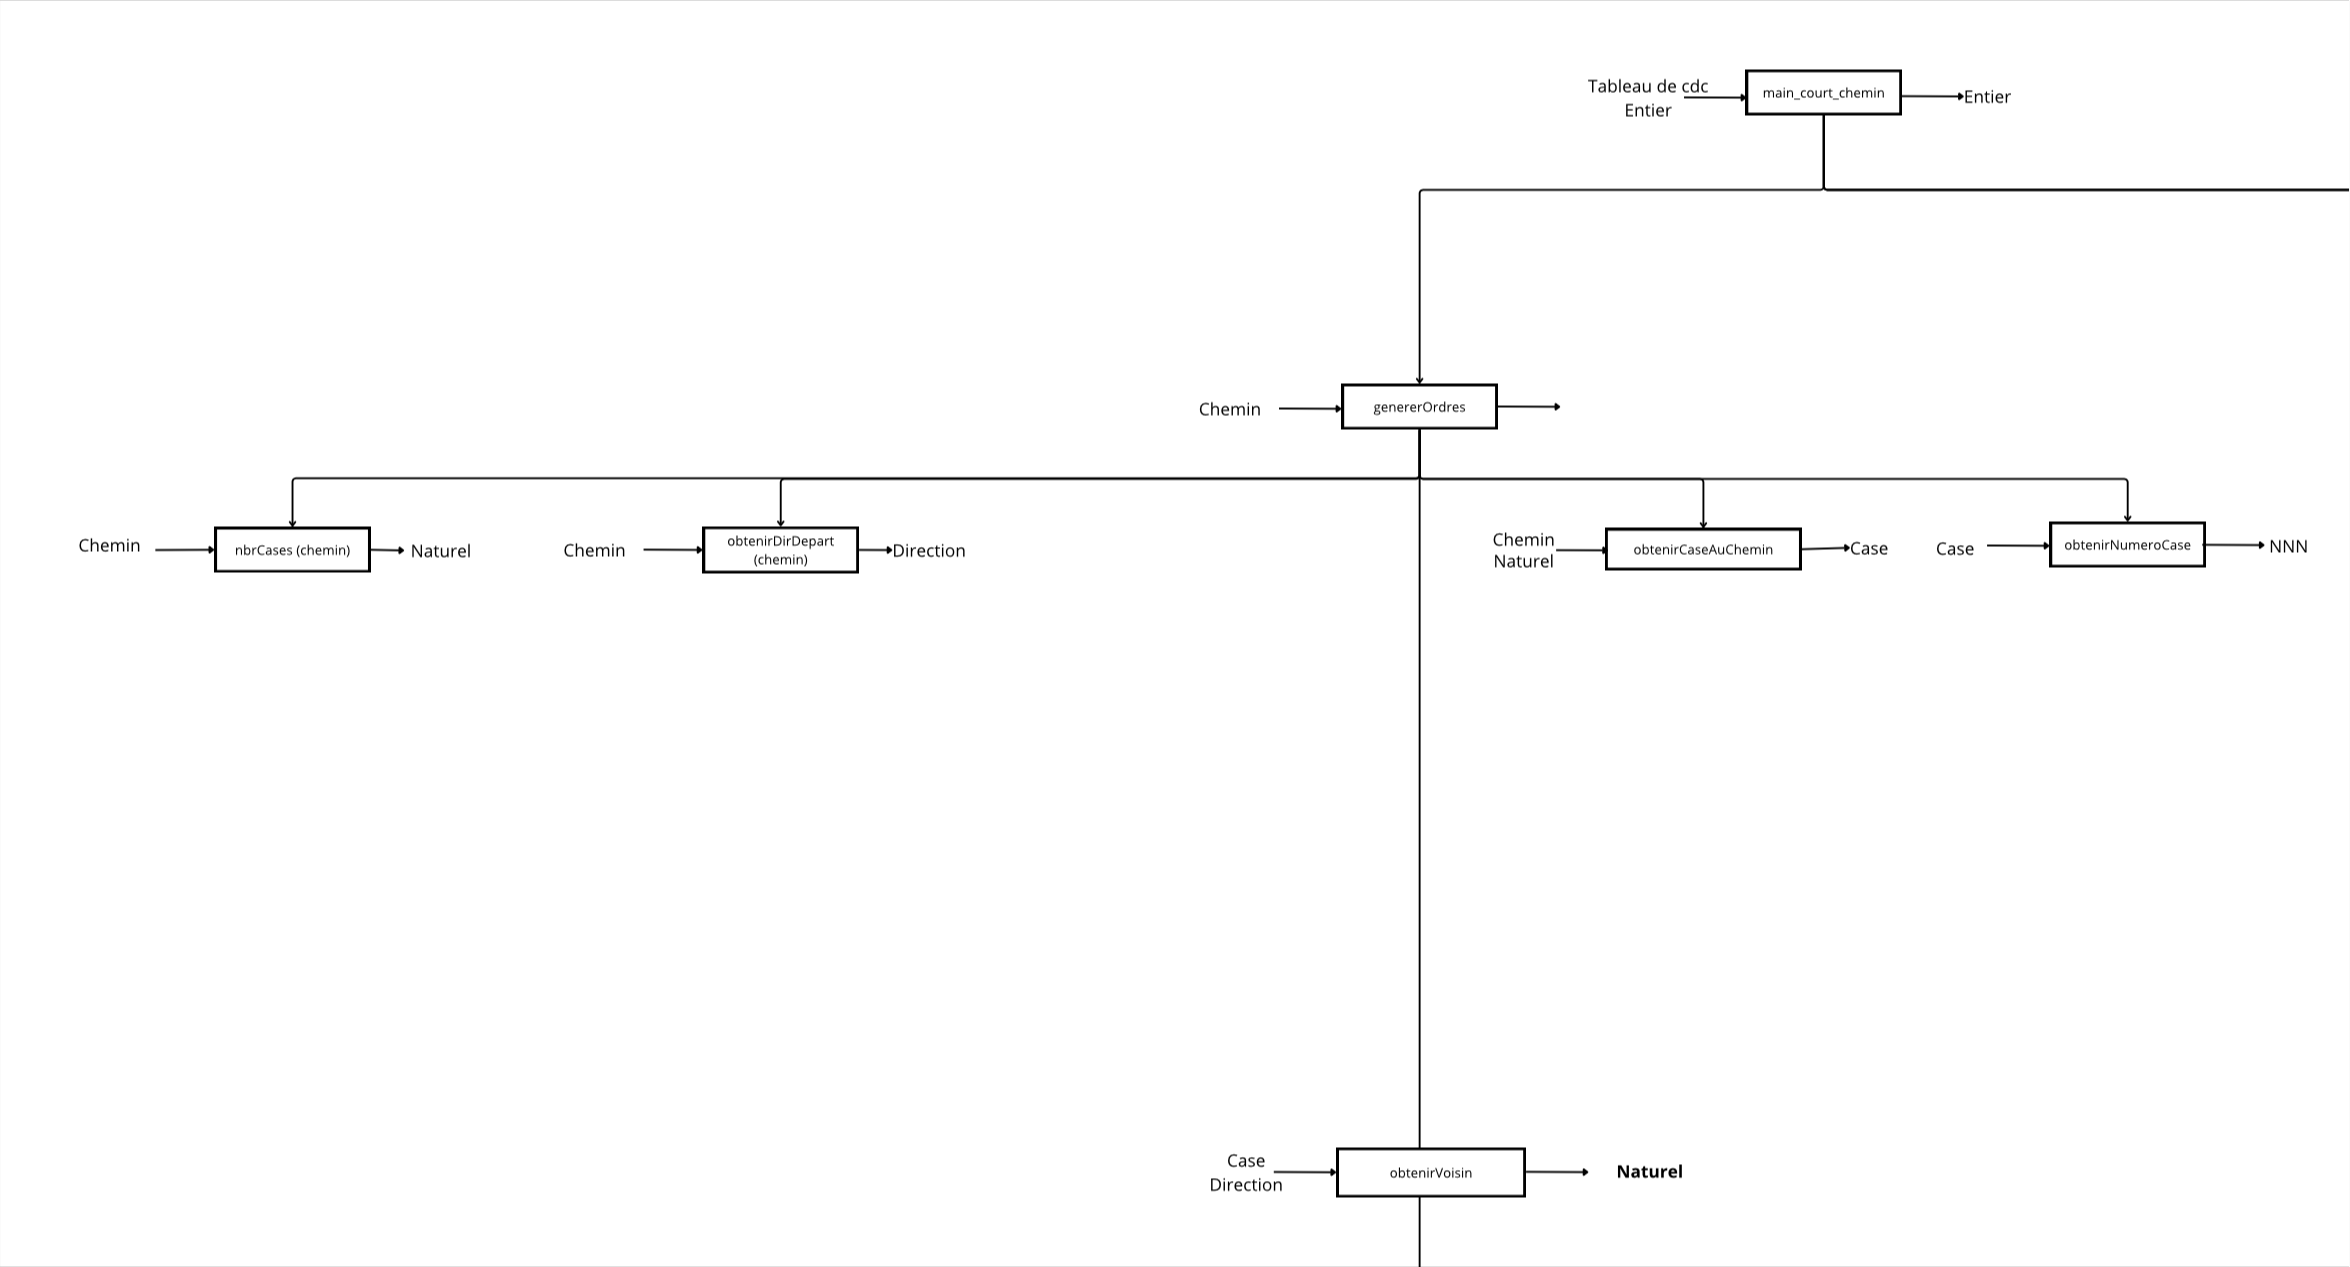
\includegraphics[width=1.0\textwidth]{image/Analyse_1.png}
    \caption{Analyse Descendante de generer\_Ordre}
    \label{fig:capteurs}
\end{figure}

\begin{figure}[H]
    \centering
    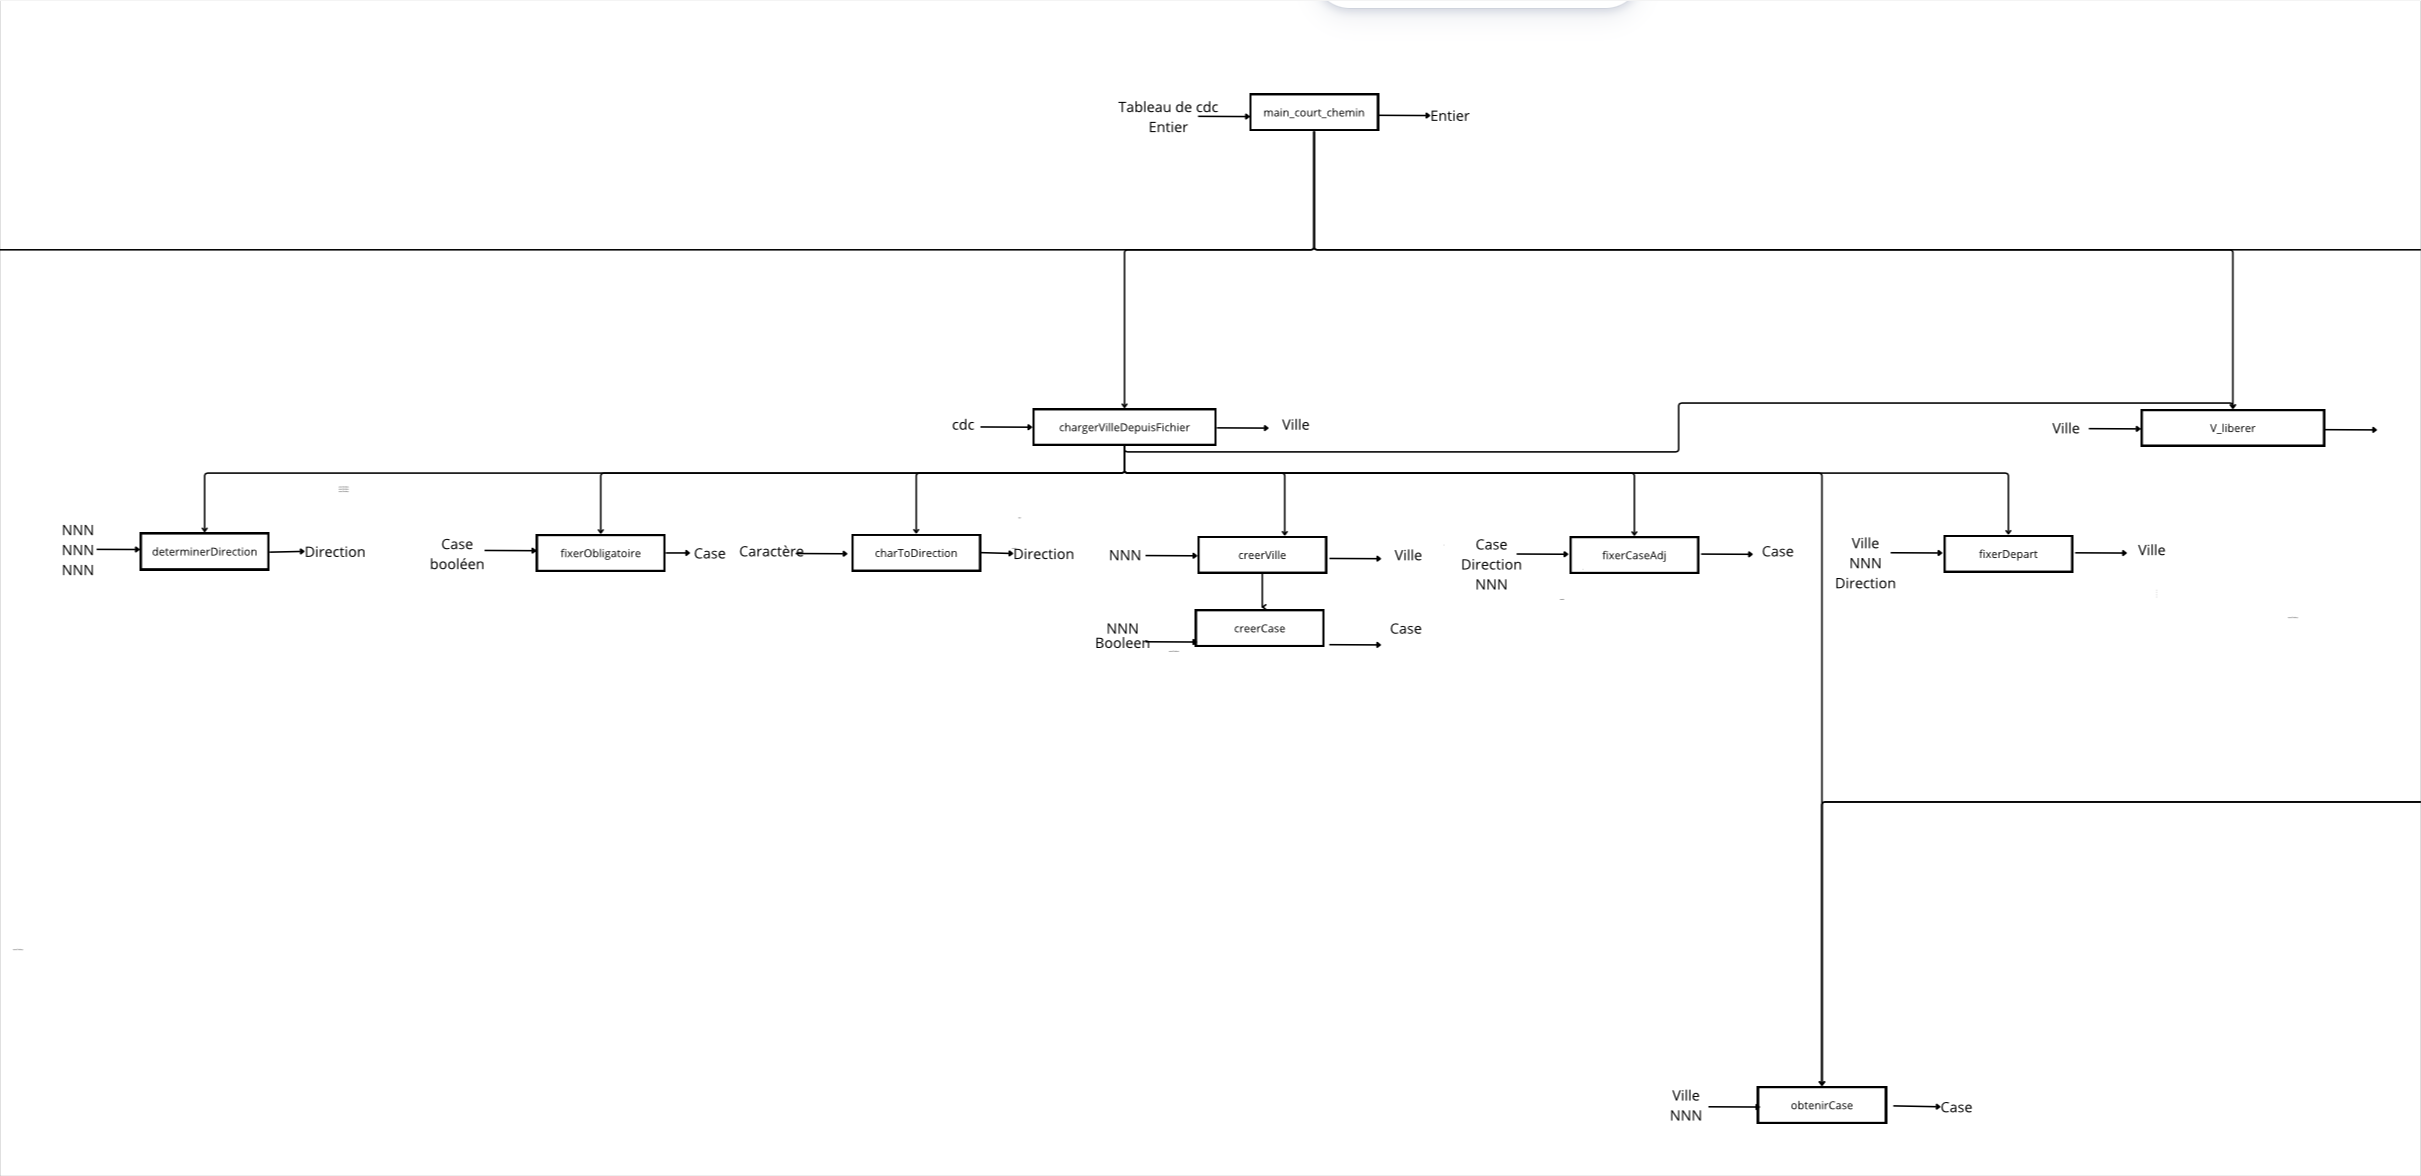
\includegraphics[width=1.0\textwidth]{image/Analyse_2.png}
    \caption{Analyse Descendante de chargerVilleDepuisFichier }
    \label{fig:capteurs}
\end{figure}

Ces dernières parties dépendent de la façon dont l'on veut résoudre le problème. 

Cette analyse descendante est pour une résolution avec le parcours en largeur.

\begin{figure}[H]
    \centering
    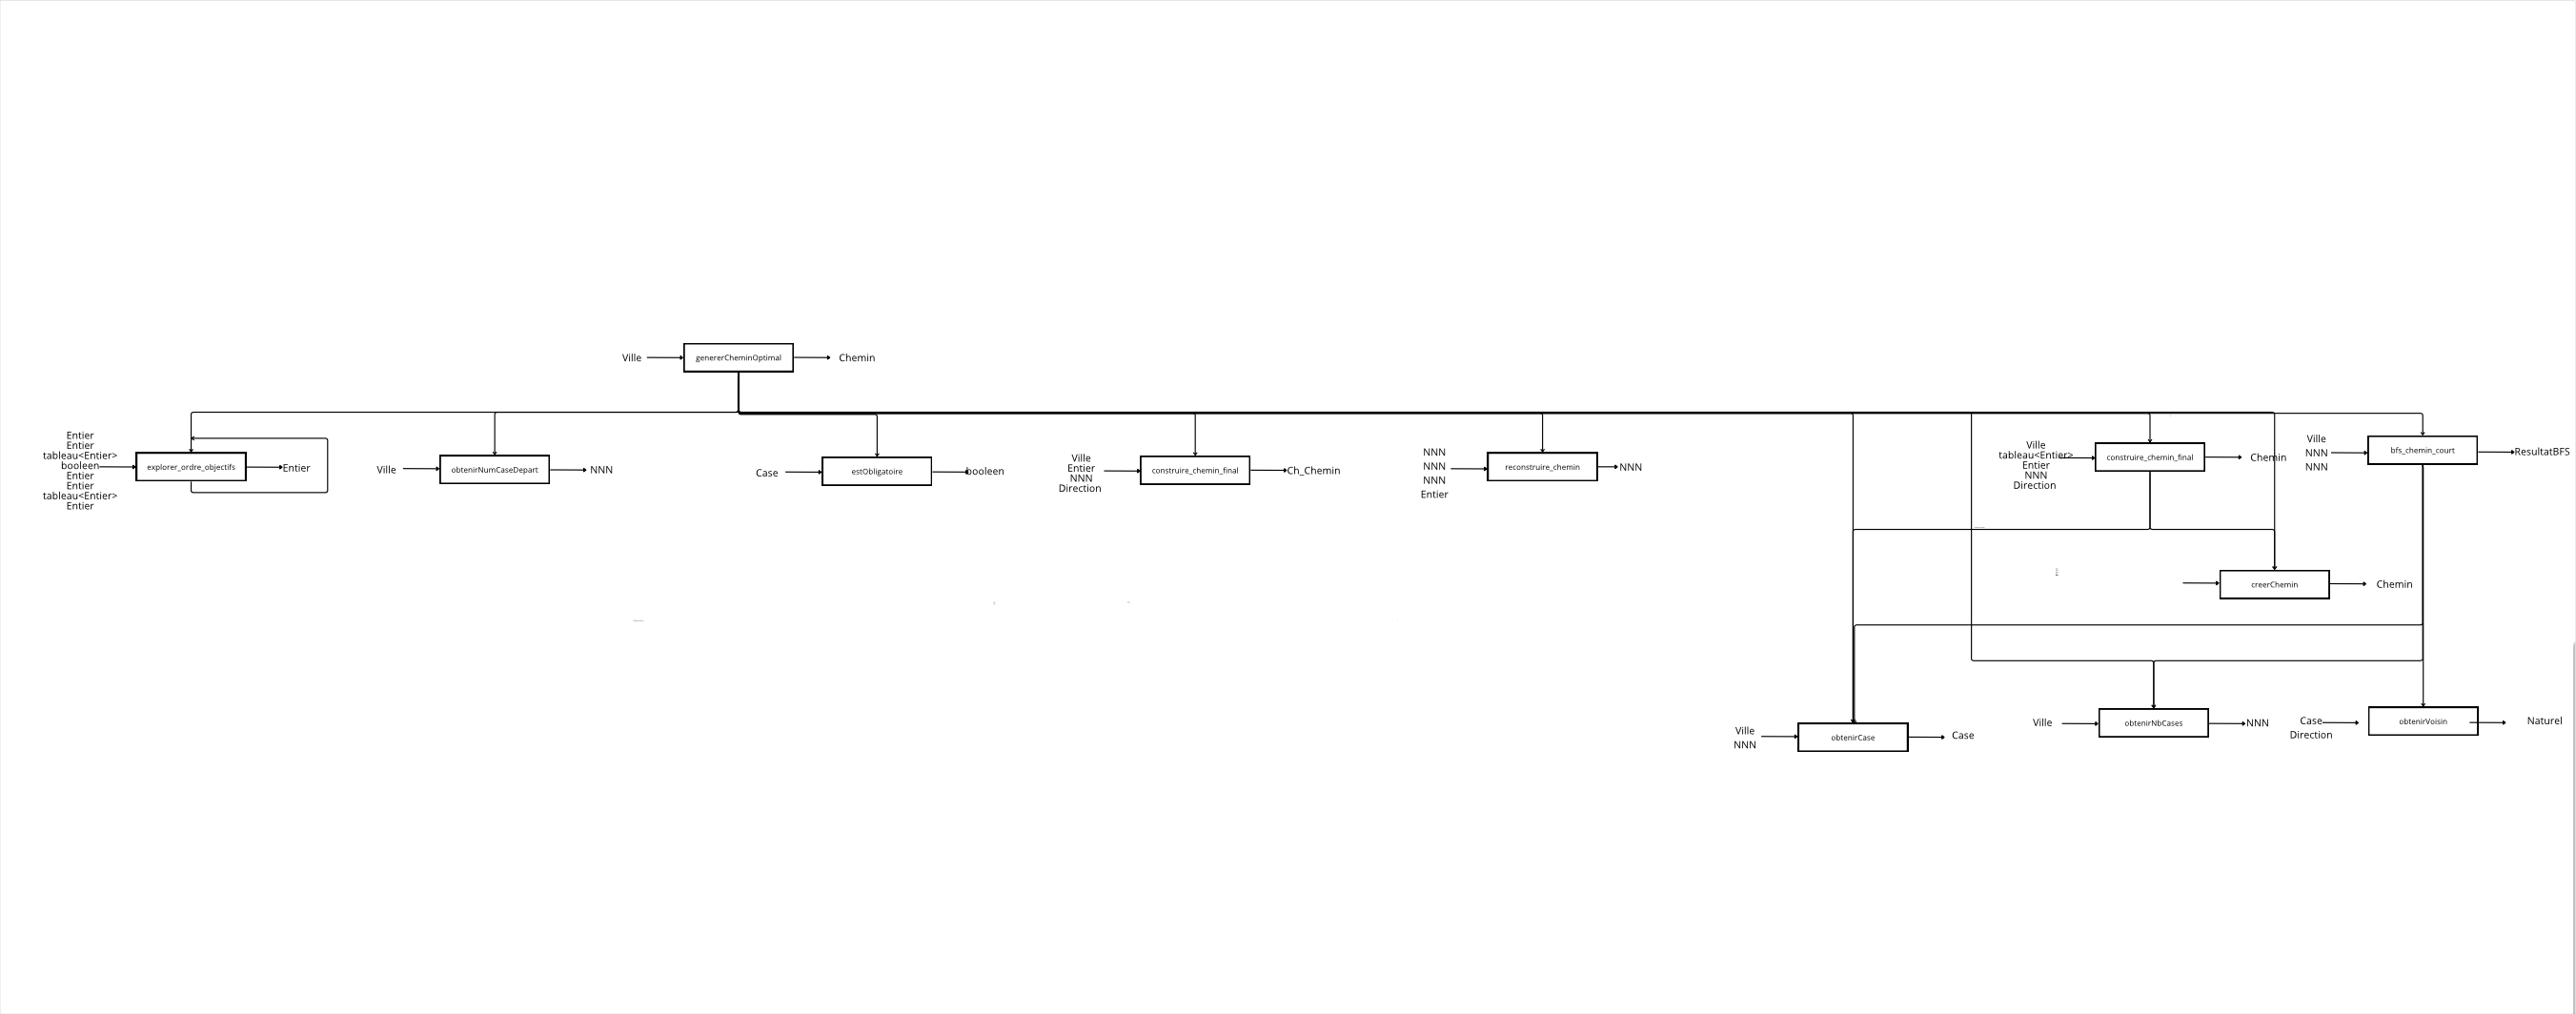
\includegraphics[width=1.0\textwidth]{image/Analyse_4.png}
    \caption{Analyse Descendante pour la résolution avec le parcours en largeur }
    \label{fig:capteurs}
\end{figure}

Cette analyse descendante est pour une résolution avec la force brute.

\begin{figure}[H]
    \centering
    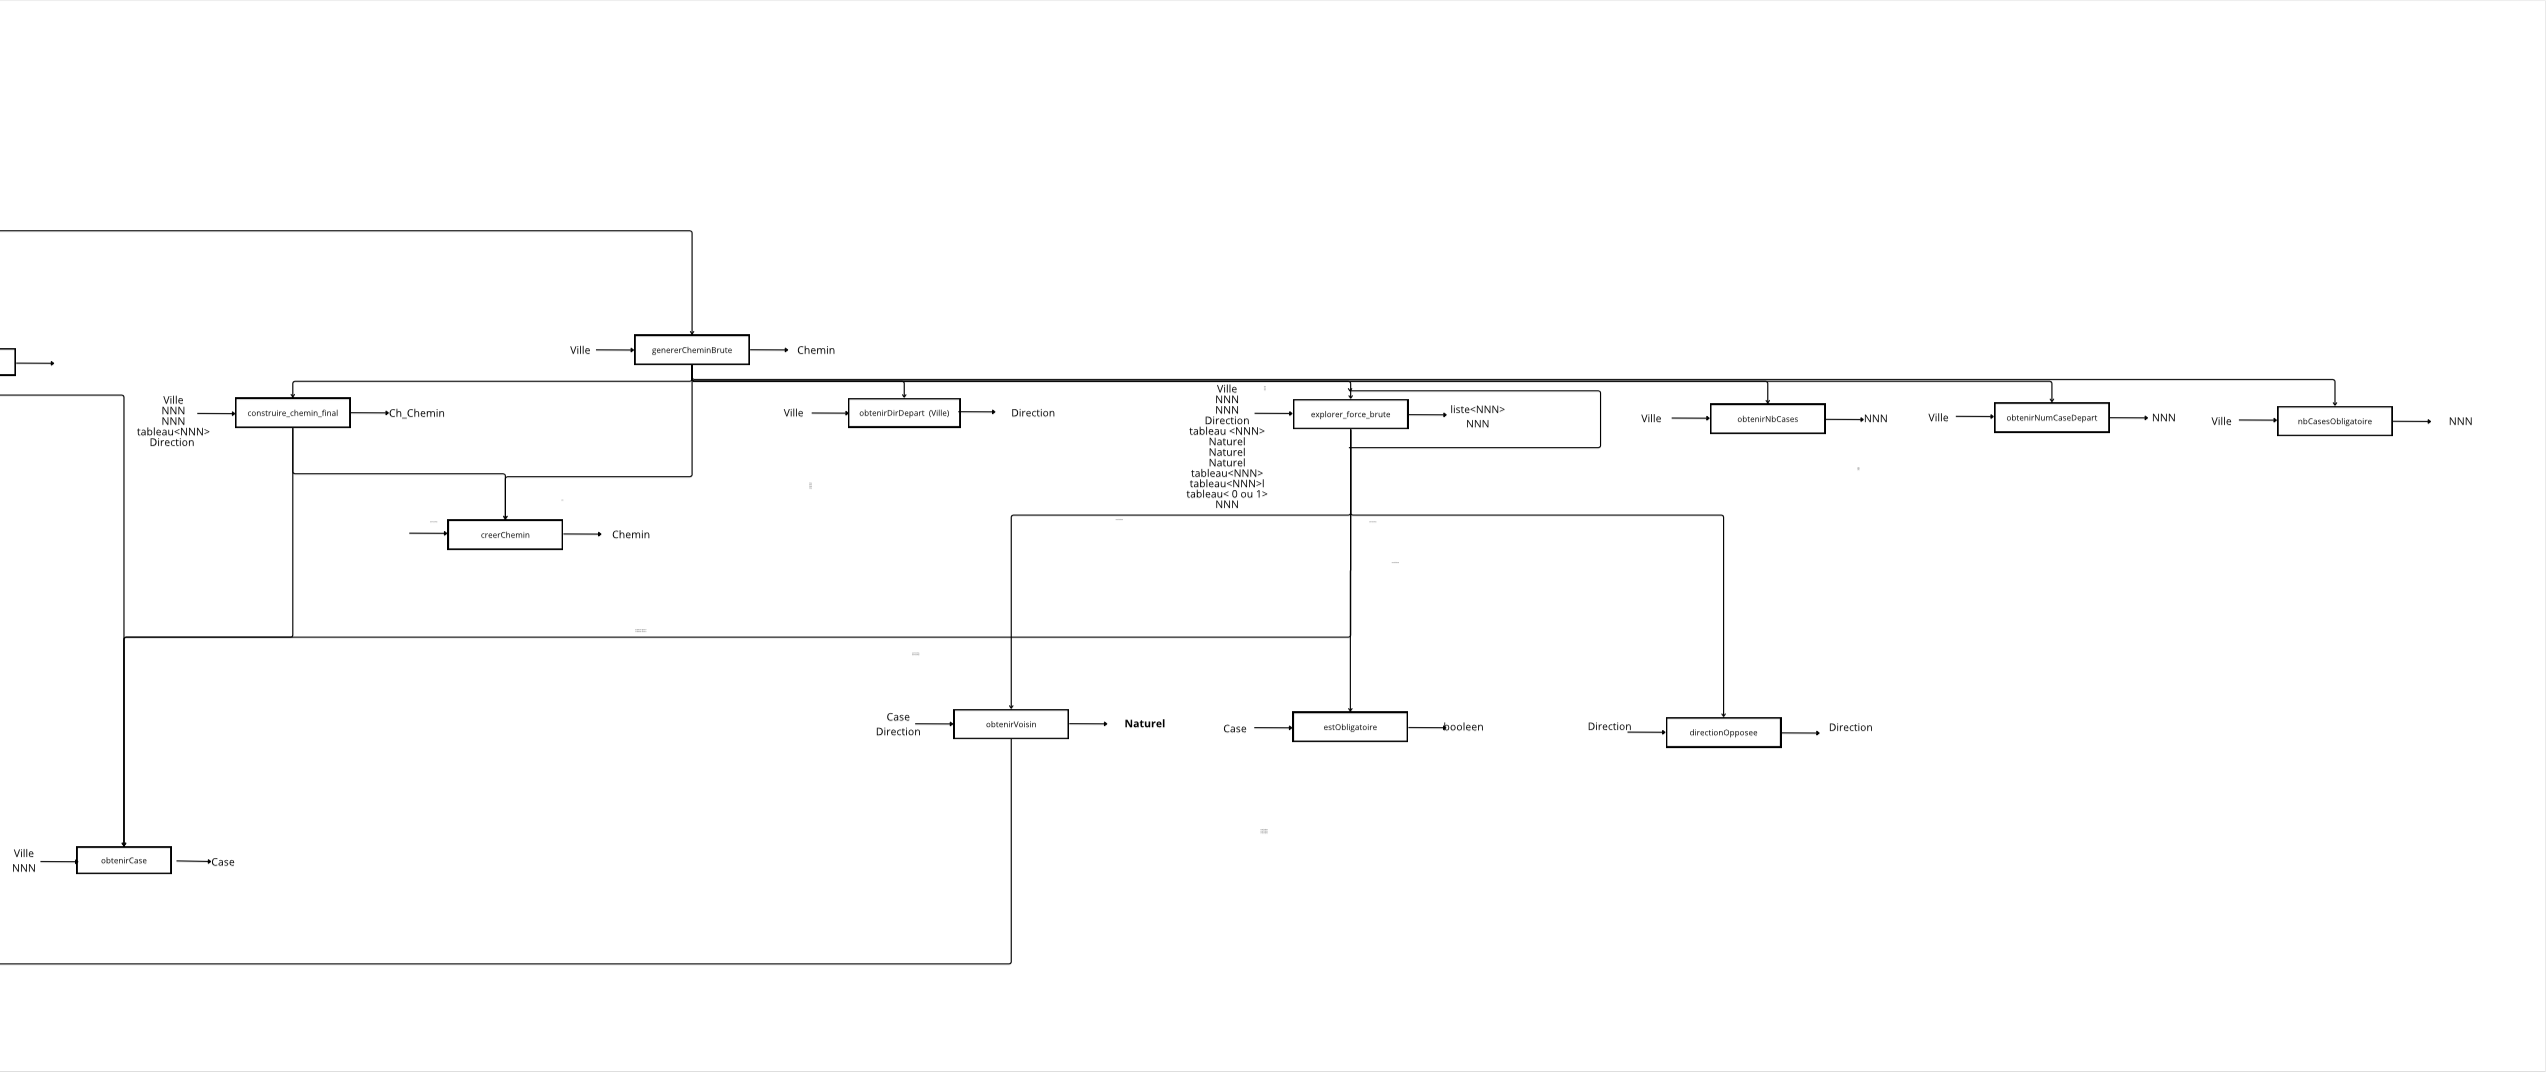
\includegraphics[width=1.0\textwidth]{image/Analyse_3.png}
    \caption{Analyse Descendante pour la résolution avec la force brute }
    \label{fig:capteurs}
\end{figure}

\begin{algorithme}
    \type{Direction}{\{NORD, EST, SUD, OUEST\}}
    \type{Commande}{\{AV, TD, TG\}}
\end{algorithme}
\subsection{TAD Ville}
\begin{tad}
    \tadNom{Ville}
    \tadDependances{\naturelNonNul, Direction, \booleen, Case}

    \begin{tadOperations}{obtenirNumCaseDepart}

        \tadOperation{creerVille}{\tadParams{\naturelNonNul}}{\tadParams{Ville}}
        
        \tadOperationAvecPreconditions{obtenirCase}{\tadParams{Ville, \naturelNonNul}}{\tadParams{Case}}
        
        \tadOperation{obtenirToutesLesCases}{\tadParams{Ville}}{\tadParams{Liste<Case>}}
        
        \tadOperationAvecPreconditions{fixerDepart}{\tadParams{Ville, \naturelNonNul, Direction}}{\tadParams{Ville}}
        
        \tadOperation{obtenirLargeur}{\tadParams{Ville}}{\tadParams{\naturelNonNul}}
        
        \tadOperation{obtenirNumCaseDepart}{\tadParams{Ville}}{\tadParams{\naturelNonNul}}
        
        \tadOperation{obtenirNbCases}{\tadParams{Ville}}{\tadParams{\naturelNonNul}}
        
        \tadOperation{obtenirDirDepart}{\tadParams{Ville}}{\tadParams{Direction}}
        
        \tadOperation{nbCasesObligatoire}{\tadParams{Ville}}{\tadParams{\naturel}}

    \end{tadOperations}
    \begin{tadPreconditions}{obtenirNumCaseDepart}

        \tadPrecondition{obtenirCase}{num\_case $\leq$ obtenirNbCases(ville)}
        \tadPrecondition{fixerDepart}{num\_case $\leq$ obtenirNbCases(ville)}
    \end{tadPreconditions}
    \begin{tadSemantiques}{obtenirNumCaseDepart}

        \tadSemantique{creeVille}{ Créer une ville dont la largeur est le paramètre largeur.}
        
        \tadSemantique{obtenirCase}{ Permet d'obtenir la case dans la ville à partir de son numéro.}
        
        \tadSemantique{ObtenirToutesLesCases}{ Permet d'obtenir le tableau contenant toutes les cases de la ville, normalement de taille largeur$^2$.}
        
        \tadSemantique{fixerDepart}{ Configure la position et l'orientation de départ dans la ville.}
        
        \tadSemantique{obtenirLargeur}{ Renvoie la largeur de la ville.}

        \tadSemantique{obtenirNumCaseDepart}{ Renvoie le numéro de la case de départ dans la ville.}

        \tadSemantique{obtenirNbCases}{ Renvoie le nombre de cases dans la ville.}
        
        \tadSemantique{obtenirDirDepart}{ Renvoie la direction de la case de départ dans la ville.}
        
         \tadSemantique{nbCasesObligatoire}{ Renvoie le nombre de cases obligatoires dans la ville.}
    \end{tadSemantiques}

    \begin{tadAxiomes}

        \tadAxiome{obtenirLargeur(creerVille(l)) = $l$}
        
        \tadAxiome{obtenirNbCases(creerVille(l)) = $l \times l$}
        
        \tadAxiome{obtenirCase(v, n) $\in$ obtenirToutesLesCases(v)}
        
        \tadAxiome{obtenirNumCaseDepart(fixerDepart(v, n, d)) = n}
        
        \tadAxiome{obtenirDirDepart(fixerDepart(v, n, d)) = d}
        
        \tadAxiome{obtenirLargeur(fixerDepart(v, n, d)) = obtenirLargeur(v)}

        \tadAxiome{nbCasesObligatoire(v) $\leq$ obtenirNbCases(v)}
    
    \end{tadAxiomes}


\end{tad}
\subsection{TAD Case}
\begin{tad}
    \tadNom{Case}
    \tadDependances{\naturel, \naturelNonNul, Direction, \booleen}

    \begin{tadOperations}{obtenirNumeroCase}

        \tadOperation{creerCase}{\tadParams{\naturelNonNul, \booleen}}{\tadParams{Case}}
        
        \tadOperation{obtenirNumeroCase}{\tadParams{Case}}{\tadParams{\naturelNonNul}}
        
        \tadOperation{estObligatoire}{\tadParams{Case}}{\tadParams{\booleen}}
        
        \tadOperation{obtenirVoisin}{\tadParams{Case, Direction}}{\tadParams{\naturel}}
        
        \tadOperation{fixerObligatoire}{\tadParams{Case, \booleen}}{\tadParams{Case}}
        
        \tadOperation{fixerCaseAdj}{\tadParams{Case, Direction, \naturelNonNul}}{\tadParams{Case}}

    \end{tadOperations}
    \begin{tadSemantiques}{obtenirNumeroCase}

        \tadSemantique{creerCase}{Crée une case identifiée par son numéro et son statut obligatoire.}
        
        \tadSemantique{obtenirNumeroCase}{Retourne le numéro unique de la case.}
        
        \tadSemantique{estObligatoire}{Indique si la case est un point de passage obligatoire.}
        
        \tadSemantique{obtenirVoisin}{Retourne le numéro de la case voisine dans la direction donnée (0 si pas de voisin).}
        
        \tadSemantique{fixerObligatoire}{Modifie le statut "obligatoire" de la case.}
        
        \tadSemantique{fixerCaseAdj}{Définit le numéro de la case voisine dans une direction donnée.}

    \end{tadSemantiques}

    \begin{tadAxiomes}

        \tadAxiome{obtenirNumeroCase(creerCase(n, obl)) = n}
        
        \tadAxiome{estObligatoire(creerCase(n, obl)) = obl}
        
        \tadAxiome{obtenirVoisin(creerCase(n, obl), d) = 0} 
        
        \tadAxiome{estObligatoire(fixerObligatoire(c, obl)) = obl}
        
        \tadAxiome{obtenirNumeroCase(fixerObligatoire(c, obl)) = obtenirNumeroCase(c)}
        
        \tadAxiome{obtenirVoisin(fixerCaseAdj(c, d, n), d) = n}
        
        \tadAxiome{obtenirNumeroCase(fixerCaseAdj(c, d, n)) = obtenirNumeroCase(c)}
        
        \tadAxiome{estObligatoire(fixerCaseAdj(c, d, n)) = estObligatoire(c)}
    
    \end{tadAxiomes}

\end{tad}


\subsection{TAD Chemin}
\begin{tad}
    \tadNom{Chemin}
    \tadDependances{\naturel, Ville, Case, Direction}

    \begin{tadOperations}{obtenirCaseAuChemin}

        \tadOperation{creerChemin}{\tadUnParam{\void}}{\tadParams{Chemin}}
        
        \tadOperation{genererCheminBrute}{\tadParams{Ville}}{\tadParams{Chemin}}

        \tadOperation{nbrCases}{\tadParams{Chemin}}{\tadParams{\naturel}}

        \tadOperation{obtenirDirDepart}{\tadParams{Chemin}}{\tadParams{Direction}}

        \tadOperationAvecPreconditions{obtenirCaseAuChemin}{\tadParams{Chemin, \naturel}}{\tadParams{Case}}

    \end{tadOperations}

    \begin{tadPreconditions}{obtenirCaseAuChemin}

        \tadPrecondition{obtenirCaseAuChemin}{obtenirCaseAuChemin(c, i) : i $\geq$ 0 et i$<$ nbrCases(chemin)}

    \end{tadPreconditions}

    \begin{tadSemantiques}{obtenirCaseAuChemin}

        \tadSemantique{creerChemin}{Initialise un chemin vide.}

        \tadSemantique{genererCheminBrute}{Génère un chemin valide dans la ville donnée en utilisant un algorithme de force brute (respectant les contraintes de passage)(genererCheminOptimal - pour l'approche BFS).}

        \tadSemantique{nbrCases}{Retourne le nombre total de cases constituant le chemin.}

        \tadSemantique{obtenirDirDepart}{Retourne la direction initiale du robot au début ce chemin.}

        \tadSemantique{obtenirCaseAuChemin}{Retourne la case située à l'index donné dans le chemin.}

    \end{tadSemantiques}

    \begin{tadAxiomes}

        \tadAxiome{nbrCases(creerChemin()) = 0}

        % Le chemin généré part de la même direction que la configuration de la ville
        \tadAxiome{obtenirDirDepart(genererCheminBrute(v)) = obtenirDirDepart(v)}

        % La première case du chemin (index 0) correspond au départ de la ville
        \tadAxiome{obtenirNumeroCase(obtenirCaseAuChemin(genererCheminBrute(v), 0)) = obtenirNumCaseDepart(v)}

    \end{tadAxiomes}

\end{tad}


\section{Conception préliminaire}
\subsection{Opérations du TAD Ville}
\begin{algorithme}
    \signatureFonction{creerVille}
        {largeur : \naturelNonNul}{Ville}

    \vspace{1.5em}

    \signatureFonctionAvecPreconditions{obtenirCase}
        {ville : Ville, num\_case : \naturelNonNul}{Case}
        {num\_case $\leq$ obtenirNbCases(ville)}

    \vspace{1.5em}

    \signatureFonction{obtenirToutesLesCases}
        {ville : Ville}{Liste<Case>}

    \vspace{1.5em}

    \signatureProcedureAvecPreconditions{fixerDepart}
        {\paramEntreeSortie{ville : Ville}, \paramEntree{num\_case : \naturelNonNul, dir : Direction}}
        {num\_case $\leq$ obtenirNbCases(ville)}

    \vspace{1.5em}

    \signatureFonction{obtenirNbCases}
        {ville : Ville}{\naturelNonNul}

    \vspace{1.5em}

    \signatureFonction{obtenirNumCaseDepart}
        {ville : Ville}{\naturelNonNul}

    \vspace{1.5em}

    \signatureFonction{obtenirDirDepart}
        {ville : Ville}{Direction}

    \vspace{1.5em}

    \signatureFonction{obtenirLargeur}
        {ville : Ville}{\naturelNonNul}

    \vspace{1.5em}

    \signatureFonction{nbCasesObligatoire}
        {ville : Ville}{\naturel}

\end{algorithme}
\subsection{Opérations du TAD Case}
\begin{algorithme}
    \signatureFonction{creerCase}
        {num : \naturelNonNul, obligatoire : \booleen}{Case}

    \vspace{1.5em}

    \signatureFonction{obtenirNumeroCase}
        {c : Case}{\naturelNonNul}

    \vspace{1.5em}

    \signatureFonction{estObligatoire}
        {c : Case}{\booleen}

    \vspace{1.5em}

    \signatureFonction{obtenirVoisin}
        {c : Case, dir : Direction}{\naturel}

    \vspace{1.5em}

    \signatureProcedure{fixerObligatoire}
        {\paramEntreeSortie{c : Case}, \paramEntree{obligatoire : \booleen}}

    \vspace{1.5em}

    \signatureProcedure{fixerCaseAdj}
        {\paramEntreeSortie{c : Case}, \paramEntree{dir : Direction, num\_case\_adj : \naturelNonNul}}

\end{algorithme}
\subsection{Opérations du TAD Chemin}
\begin{algorithme}
    \signatureFonction{creerChemin}
        {}{\typePointeur{Chemin}}

    \vspace{1.5em}

    \signatureFonction{genererCheminBrute}
        {ville : Ville}{\typePointeur{Chemin}}

    \vspace{1.5em}

    \signatureFonction{nbrCases}
        {chemin : Chemin}{\naturel}

    \vspace{1.5em}

    \signatureFonction{obtenirDirDepart}
        {chemin : Chemin}{Direction}

    \vspace{1.5em}

    \signatureFonctionAvecPreconditions{obtenirCaseAuChemin}
        {chemin : Chemin, i : \naturel}{Case}
        {i $\geq$ 0 et i $<$ nbrCases(chemin)}

\end{algorithme}
\subsection{IHM}
Les focntions afficherChemin et afficherVille ne sont pas utilisées pour le projet entier mais elles nous ont servi lorsqu'on a testé des différentes villes et algorithmes qui permettaient de calculer un plus court chemin. 

\vspace{1cm}

\begin{algorithme}
    \signatureFonction{chargerVilleDepuisFichier}
        {nom\_fichier : \chaine}{Ville}

    \vspace{1.5em}

    \signatureProcedure{afficherChemin}
        {\paramEntree{chemin : Chemin}}

    \vspace{1.5em}

    \signatureProcedure{afficherVille}
        {\paramEntree{ville : Ville}}

    \vspace{1.5em}

    \signatureProcedure{genererOrdres}
        {\paramEntree{chemin : Chemin}}

\end{algorithme}
\subsection{Logique métier}
\begin{algorithme}
    \signatureFonction{directionOpposee}
        {direction : Direction}{Direction}
        {}
\end{algorithme}

\section{Conception détaillée}
\subsection{Structures}
\begin{algorithme}
    \begin{itemize}
        \item[$\bullet$] 
        \begin{enregistrement}{Case}
            \champEnregistrement{numero\_case}{\naturelNonNul}
            \champEnregistrement{est\_obligatoire}{\booleen} 
            \champEnregistrement{cases\_adjacents}{\tableauUneDimension{4}{de }{\naturelNonNul}}
        \end{enregistrement}

        \item[$\bullet$] 
        \begin{enregistrement}{Chemin}
            \champEnregistrement{nb\_cases}{\naturelNonNul}  
            \champEnregistrement{tab\_cases}{\tableauUneDimension{nb\_cases}{de}{Case}}
            \champEnregistrement{num\_case\_depart}{\naturelNonNul}
            \champEnregistrement{dir\_depart}{Direction}        
        \end{enregistrement}

        \item[$\bullet$] 
        \begin{enregistrement}{Ville}
            \champEnregistrement{largeur}{\naturel}             
            \champEnregistrement{nb\_cases}{\naturel}          
            \champEnregistrement{tab\_cases}{\tableauUneDimension{nb\_cases}{de}{Case}} 
            \champEnregistrement{num\_case\_depart}{\naturel}  
            \champEnregistrement{dir\_depart}{Direction}        
        \end{enregistrement}
        
    \end{itemize}
\end{algorithme}
\subsection{Pseudo code du plus court chemin par parcours en largeur}

L'approche BFS génère deux informations distinctes et nécessaires : la distance minimale (un naturel) qui valide l'existence d'un chemin, et la trace des prédécesseurs (un tableau) qui permet de remonter de l'arrivée vers le départ pour reconstituer l'itinéraire. Le langage C ne permettant pas le retour de valeurs multiples, l'encapsulation de ces deux données dans la structure ResultatBFS permet de récupérer l'intégralité du résultat de l'exploration en une seule opération.

Nous avons donc ajouté une structure afin de nous aider dans notre démarche.

\item[$\bullet$] 
        \begin{enregistrement}{ResultatBFS}
            \champEnregistrement{Distance}{\naturel}             
            \champEnregistrement{predecesseurs}{\tableauUneDimension{ }de {\naturelNonNul}    }      
        \end{enregistrement}
        
\vspace{1cm}

\begin{algorithme}
    \fonction{genererCheminOptimal}
        {v : Ville}
        {Chemin}
        {nb\_cases, depart, nb\_objectifs, i ,j , k ,l, taille\_max , idx\_depart , idx\_arrivee : \naturelNonNul \\
        longueur\_totale, longueur\_segment, debut  : \naturel\\
        min\_cout  : \entier\\
        distances : \tableauDeuxDimensions{ } { } {de} {\entier} \\
        objectifs , sequence\_temp, meilleure\_sequence, chemin\_final, segment : \tableauUneDimension{ } de {\naturelNonNul} \\
        visites : \tableauUneDimension{ } de {\bool}\\
        predecesseurs : \tableauDeuxDimensions{ } { } {de} {\naturel} \\
        resBFS : ResultatBFS \\
        resultat : Chemin \\
        } 
        {
        \sialors{v = \motclefPointeurNULL}
            {\retourner{creerChemin()}}

        \affecter{nb\_cases}{obtenirNbCases(v)}
        \affecter{depart}{obtenirNumCaseDepart(v)}

        \affecter{objectifs}{allouer(nb\_cases + 1)}
        \affecter{objectifs[0]}{depart}
        \affecter{nb\_objectifs}{1}

        \pour{i}{1}{nb\_cases}{}{
            \affecter{c}{obtenirCase(v, i)}
            \sialors{estObligatoire(c) et i $\neq$ depart}
            {
                \affecter{objectifs[nb\_objectifs]}{i}
                \affecter{nb\_objectifs}{nb\_objectifs + 1}
            }
        }

        \sialors{nb\_objectifs $\leq$ 1}
        {
            \affecter{resultat}{construire\_chemin\_final(v, depart, 0, depart, obtenirDirDepart(v))}
            \instruction{desallouer(objectifs)}
            \retourner{resultat}
        }

        \affecter{distances}{allouerMatrice(nb\_objectifs, nb\_objectifs)}
        \affecter{predecesseurs}{allouerMatrice(nb\_objectifs, nb\_objectifs)}

        \pour{i}{0}{nb\_objectifs - 1}{}{
            \affecter{distances[i]}{allouer(nb\_objectifs)}
            \affecter{predecesseurs[i]}{allouer(nb\_objectifs)}

            \pour{j}{0}{nb\_objectifs - 1}{}{
                \sialorssinon{i = j}
                {
                    \affecter{distances[i][j]}{0}
                    \affecter{predecesseurs[i][j]}{\motclefPointeurNULL}
                }
                {
                    \affecter{resBFS}{bfs\_chemin\_court(v, objectifs[i], objectifs[j])}
                    \affecter{distances[i][j]}{resBFS.distance}
                    \affecter{predecesseurs[i][j]}{resBFS.predecesseurs}

                    \sialors{resBFS.distance = {\infty }}
                    {
                        \instruction{desallouer(objectifs)}
                        \pour{k}{0}{i}{}{
                            \pour{l}{0}{nb\_objectifs - 1}{}{
                                \sialors{predecesseurs[k][l] $\neq$ \motclefPointeurNULL}
                                    {\instruction{desallouer(predecesseurs[k][l])}}
                            }
                            \instruction{desallouer(predecesseurs[k])}
                            \instruction{desallouer(distances[k])}
                        }
                        \instruction{desallouer(predecesseurs)}
                        \instruction{desallouer(distances)}
                        \retourner{creerChemin()}
                    }
                }
            }
        }

        \affecter{sequence\_temp}{allouer(nb\_objectifs)}
        \affecter{meilleure\_sequence}{allouer(nb\_objectifs)}
        \affecter{visites}{allouer(nb\_objectifs)}
        \affecter{min\_cout}{\infty}

        \affecter{sequence\_temp[0]}{0}
        \affecter{visites[0]}{vrai}

        \instruction{explorer\_ordre\_objectifs(1, nb\_objectifs,
                     sequence\_temp, visites, 0,
                     distances, meilleure\_sequence, \&min\_cout)}

        \sialors{min\_cout = \infty}
        {
            \instruction{desallouer(sequence\_temp)}
            \instruction{desallouer(meilleure\_sequence)}
            \instruction{desallouer(visites)}
            \instruction{desallouer(objectifs)}
            \pour{i}{0}{nb\_objectifs - 1}{}{
                \pour{j}{0}{nb\_objectifs - 1}{}{
                    \sialors{predecesseurs[i][j] $\neq$ \motclefPointeurNULL}
                        {\instruction{desallouer(predecesseurs[i][j])}}
                }
                \instruction{desallouer(predecesseurs[i])}
                \instruction{desallouer(distances[i])}
            }
            \instruction{desallouer(predecesseurs)}
            \instruction{desallouer(distances)}
            \retourner{creerChemin()}
        }

        \affecter{taille\_max}{2 \times {nb\_cases} + 2}
        \affecter{chemin\_final}{allouer(taille\_max)}
        \affecter{longueur\_totale}{0}

        \pour{i}{0}{nb\_objectifs - 1}{}{
            \affecter{idx\_depart}{meilleure\_sequence[i]}
            \sialorssinon{i = nb\_objectifs - 1}
                {\affecter{idx\_arrivee}{0}}
                {\affecter{idx\_arrivee}{meilleure\_sequence[i + 1]}}

            \affecter{segment}{allouer(nb\_cases + 1)}
            \affecter{longueur\_segment}{reconstruire\_chemin(
                objectifs[idx\_depart],
                objectifs[idx\_arrivee],
                predecesseurs[idx\_depart][idx\_arrivee],
                segment)}

            \sialors{longueur\_segment < 0}
            {
                \instruction{desallouer(segment)}
                \continuer
            }

            \sialorssinon{i = 0}
                {\affecter{debut}{0}}
                {\affecter{debut}{1}}

            \pour{j}{debut}{longueur\_segment}{}{
                \affecter{chemin\_final[longueur\_totale]}{segment[j]}
                \affecter{longueur\_totale}{longueur\_totale + 1}
            }

            \instruction{desallouer(segment)}
        }

        \affecter{resultat}{construire\_chemin\_final(
            v, chemin\_final, longueur\_totale - 1,
            depart, obtenirDirDepart(v))}

        \instruction{desallouer(objectifs)}
        \instruction{desallouer(chemin\_final)}
        \instruction{desallouer(sequence\_temp)}
        \instruction{desallouer(meilleure\_sequence)}
        \instruction{desallouer(visites)}

        \pour{i}{0}{nb\_objectifs - 1}{}{
            \pour{j}{0}{nb\_objectifs - 1}{}{
                \sialors{i $\neq$ j et predecesseurs[i][j] $\neq$ \motclefPointeurNULL}
                    {\instruction{desallouer(predecesseurs[i][j])}}
            }
            \instruction{desallouer(predecesseurs[i])}
            \instruction{desallouer(distances[i])}
        }

        \instruction{desallouer(predecesseurs)}
        \instruction{desallouer(distances)}

        \retourner{resultat}
    }
\end{algorithme}





\subsection{Pseudo code de la fonction explorer ordre objectifs }
\begin{algorithme}
    \procedure{explorer\_ordre\_objectifs}
        {
            \paramEntree{position : \naturel}, 
            \paramEntree{nb\_obj : \naturelNonNul}, 
            \paramEntreeSortie{sequence\_temp : \tableauUneDimension{}{de}{\naturel}}, 
            \paramEntreeSortie{visites : \tableauUneDimension{}{de}{\booleen}}, 
            \paramEntree{cout\_actuel : \naturel}, 
            \paramEntree{distances : \tableauDeuxDimensions{}{}{de}{\naturel}}, 
            \paramEntreeSortie{meilleure\_sequence : \tableauUneDimension{}{de}{\naturel}}, 
            \paramEntreeSortie{min\_cout : \entier} 
        }
        {
            cout\_retour, cout\_total, cout\_segment, i : \naturel
        }
    {
        \sialors{cout\_actuel < \valeurPointeur{min\_cout}} 
        {
            \sialorssinon{position = nb\_obj}
            {
                \affecter{cout\_retour}{distances[sequence\_temp[nb\_obj - 1]][0]}
                
                \sialors{cout\_retour \neq \infty}
                {
                    \affecter{cout\_total}{cout\_actuel + cout\_retour}

                    \sialors{cout\_total < \valeurPointeur{min\_cout}}
                    {
                        \affecter{\valeurPointeur{min\_cout}}{cout\_total}

                        \pour{i}{0}{nb\_obj - 1}{}{
                            \affecter{meilleure\_sequence[i]}{sequence\_temp[i]}
                        }
                    }
                }
            }
            {
                \pour{i}{1}{nb\_obj - 1}{}{
                    \sialors{non visites[i]}
                    {
                        \affecter{cout\_segment}{distances[sequence\_temp[position - 1]][i]}
                        \sialors{cout\_segment \neq \infty}
                        {
                            \affecter{visites[i]}{vrai}
                            \affecter{sequence\_temp[position]}{i}
                            \instruction{explorer\_ordre\_objectifs(
                                position + 1, nb\_obj,
                                sequence\_temp, visites,
                                cout\_actuel + cout\_segment,
                                distances,
                                meilleure\_sequence,
                                min\_cout)}

                            \affecter{visites[i]}{faux}
                        }
                    }
                }
            }
        }
    }
\end{algorithme}


\subsection{Pseudo code de la fonction reconstruire chemin}
\begin{algorithme}
    \procedure{reconstruire\_chemin}
        {
            \paramEntree{depart : \naturelNonNul},
            \paramEntree{arrivee : \naturelNonNul},
            \paramEntree{predecesseurs : \tableauUneDimension{}{de}{\naturel}},
            \paramEntreeSortie{chemin\_sortie : \tableauUneDimension{}{de}{\naturel}},
            \paramEntreeSortie{longueur\_resultat : \entier}
        }
        {
            longueur : \entier \\
            actuel : \naturel \\
            i, temp : \entier
        }
    {
        \sialorssinon{ (predecesseurs = \motclefPointeurNULL) ou ((predecesseurs[arrivee] = 0) et (depart \neq arrivee)) }
        {
            \affecter{\valeurPointeur{longueur\_resultat}}{-1}
        }
        {
            \affecter{longueur}{0}
            \affecter{actuel}{arrivee}

            \tantque{actuel \neq 0}
            {
                \affecter{chemin\_sortie[longueur]}{actuel}
                \affecter{longueur}{longueur + 1}

                \sialorssinon{actuel = depart}
                {
                    \affecter{actuel}{0}
                }
                {
                    \affecter{actuel}{predecesseurs[actuel]}
                }
            }

            \pour{i}{0}{(longueur / 2) - 1}{}{
                \affecter{temp}{chemin\_sortie[i]}
                \affecter{chemin\_sortie[i]}{chemin\_sortie[longueur - 1 - i]}
                \affecter{chemin\_sortie[longueur - 1 - i]}{temp}
            }

            \affecter{\valeurPointeur{longueur\_resultat}}{longueur - 1}
        }
    }
\end{algorithme}

\subsection{Pseudo code de la fonction  construire chemin final}
\begin{algorithme}
    \fonction{construire\_chemin\_final}
        {v : Ville,
         ids\_chemin : \tableauUneDimension{}{de}{\entier},
         longueur : \entier,
         depart : \naturelNonNul,
         dir : Direction}
        {Chemin}
        {c : Chemin \\
         i : \entier \\
         case\_orig : Case}
    {
        \affecter{c}{creerChemin()}

        \affecter{c.nb\_cases}{longueur}
        \affecter{c.num\_case\_depart}{depart}
        \affecter{c.dir\_depart}{dir}

        \affecter{c.tab\_cases}{allouer(longueur + 1)}

        \pour{i}{0}{longueur}{}{
            \affecter{case\_orig}{obtenirCase(v, ids\_chemin[i])}
            \sialors{case\_orig $\neq$ \motclefPointeurNULL}
            {
                \affecter{c.tab\_cases[i]}{\valeurPointeur{case\_orig}}
            }
        }

        \retourner{c}
    }
\end{algorithme}

\subsection{Pseudo code de la fonction bfs chemin court}
\begin{algorithme}
    \fonction{bfs\_chemin\_court}
        {v : Ville,
         depart : \naturelNonNul,
         arrivee : \naturelNonNul}
        {ResultatBFS}
        {resultat : ResultatBFS \\
         nb\_cases : \naturel \\
         distances : \tableauUneDimension{}{de}{\entier} \\
         file : \tableauUneDimension{}{de}{\naturel} \\
         debut, fin, i : \entier \\
         case\_actuelle, voisin : \naturel \\
         ptr\_case : Case \\
         trouve : \booleen}
    {
        \affecter{resultat.distance}{\infty}
        \affecter{resultat.predecesseurs}{\motclefPointeurNULL}
        \affecter{trouve}{faux}

        \sialors{depart = arrivee}
        {
            \affecter{resultat.distance}{0}
            \retourner{resultat}
        }

        \affecter{nb\_cases}{obtenirNbCases(v)}
        \affecter{resultat.predecesseurs}{allouer(nb\_cases + 1)}
        \affecter{distances}{allouer(nb\_cases + 1)}
        \affecter{file}{allouer(nb\_cases + 1)}

        \pour{i}{0}{nb\_cases}{}{
            \affecter{distances[i]}{\infty}
        }

        \affecter{debut}{0}
        \affecter{fin}{0}
        \affecter{distances[depart]}{0}
        \affecter{file[fin]}{depart}
        \affecter{fin}{fin + 1}

        \tantque{debut < fin \textbf{et} non trouve}
        {
            \affecter{case\_actuelle}{file[debut]}
            \affecter{debut}{debut + 1}

            \sialorssinon{case\_actuelle = arrivee}
            {
                \affecter{resultat.distance}{distances[arrivee]}
                \affecter{trouve}{vrai}
            }
            {
                \affecter{ptr\_case}{obtenirCase(v, case\_actuelle)}

                \sialors{ptr\_case $\neq$ \motclefPointeurNULL}
                {
                    \pour{i}{0}{3}{}{
                        \affecter{voisin}{
                            obtenirVoisin(
                                \valeurPointeur{ptr\_case},
                                entierVersDirection(i))
                        }

                        \sialors{
                            voisin $\neq$ 0
                            \textbf{et}
                            distances[voisin] = \infty
                        }
                        {
                            \affecter{distances[voisin]}
                                     {distances[case\_actuelle] + 1}
                            \affecter{resultat.predecesseurs[voisin]}
                                     {case\_actuelle}
                            \affecter{file[fin]}{voisin}
                            \affecter{fin}{fin + 1}
                        }
                    }
                }
            }
        }

        \sialors{non trouve}
        {
            \instruction{desallouer(resultat.predecesseurs)}
            \affecter{resultat.predecesseurs}{\motclefPointeurNULL}
        }

        \instruction{desallouer(file)}
        \instruction{desallouer(distances)}

        \retourner{resultat}
    }
\end{algorithme}




\subsection{Pseudo code du plus court chemin par force brute}
\begin{algorithme}

\procedure{ExplorerForceBrute}
{
    \paramEntree{v : Ville},
    \paramEntree{idCase : \naturelNonNul},
    \paramEntree{idDepart : \naturelNonNul},
    \paramEntree{dirActuelle : Direction},
    \paramEntreeSortie{cheminTemp : \tableauUneDimension{}{de}{\naturel}},
    \paramEntree{profondeur : \naturel},
    \paramEntree{objTrouves : \naturel},
    \paramEntree{objTotal : \naturel},
    \paramEntreeSortie{meilleurChemin : \tableauUneDimension{}{de}{\naturel}},
    \paramEntreeSortie{minLen : \entier},
    \paramEntreeSortie{objCollectes : \tableauUneDimension{}{de}{\booleen}},
    \paramEntree{tailleMax : \naturel}
}
{
    cActuelle : Case \\
    voisinId : \naturel \\
    dir, i : \entier \\
    aRamasseObjet : \booleen
}
{
    \sialors{profondeur < tailleMax \textbf{ et } profondeur < minLen}
    {
        \affecter{cActuelle}{obtenirCase(v, idCase)}

        \sialors{cActuelle \neq \motclefPointeurNULL}
        {
            \affecter{cheminTemp[profondeur]}{idCase}
            \affecter{aRamasseObjet}{faux}


            \sialors{estObligatoire(cActuelle) \textbf{ et } non objCollectes[idCase]}
            {
                \affecter{objCollectes[idCase]}{vrai}
                \affecter{objTrouves}{objTrouves + 1}
                \affecter{aRamasseObjet}{vrai}
            }


            \sialors{idCase = idDepart \textbf{ et } profondeur > 0 \textbf{ et } objTrouves \geq objTotal}
            {
                \affecter{minLen}{profondeur}
                \pour{i}{0}{profondeur}{}{
                    \affecter{meilleurChemin[i]}{cheminTemp[i]}
                }
            }

            \pour{dir}{0}{3}{}{
                \sialors{entierVersDirection(dir) \neq directionOpposee(dirActuelle)}
                {
                    \affecter{voisinId}{obtenirVoisin(cActuelle, entierVersDirection(dir))}
                    \sialors{voisinId \neq 0}
                    {
                        \instruction{ExplorerForceBrute(
                            v,
                            voisinId,
                            idDepart,
                            entierVersDirection(dir),
                            cheminTemp,
                            profondeur + 1,
                            objTrouves,
                            objTotal,
                            meilleurChemin,
                            minLen,
                            objCollectes,
                            tailleMax
                        )}
                    }
                }
            }

            \sialors{aRamasseObjet}
            {
                \affecter{objCollectes[idCase]}{faux}
            }
        }
    }
}


\vspace{1cm}

\begin{algorithme}
\fonction{GenererCheminBrute}
{v : Ville}
{Chemin}
{
    nbCases, departId, objTotal, tailleMax, minLen : Naturel \\
    dirDepart : Direction \\
    cheminTemp, meilleurChemin : \tableauUneDimension{}{de}{Naturel} \\
    objectifs : \tableauUneDimension{}{de}{Naturel} \\
    resultat : Chemin
}
{
    \sialors{v = \motclefPointeurNULL}
    {
        \retourner{creerCheminVide()}
    }

    \affecter{nbCases}{obtenirNbCases(v)}

    \affecter{tailleMax}{(nbCases * 2) + 2}
    \sialors{tailleMax < 4}
    {
        \affecter{tailleMax}{4}
    }

    \affecter{departId}{obtenirNumCaseDepart(v)}
    \affecter{dirDepart}{obtenirDirDepart(v)}
    \affecter{objTotal}{nbCasesObligatoire(v)}

    \allouer{cheminTemp, tailleMax}\\
    \allouer{meilleurChemin, tailleMax}\\
    \allouer{objectifs, nbCases + 1}\\

    \affecter{minLen}{TAILLE\_MAX\_CHEMIN}

    \instruction{ExplorerForceBrute(
        v,
        departId,
        departId,
        dirDepart,
        cheminTemp,
        0,
        0,
        objTotal,
        meilleurChemin,
        minLen,
        objectifs,
        tailleMax
    )}

    \affecter{resultat}{construireCheminFinal(
        v,
        meilleurChemin,
        minLen,
        departId,
        dirDepart
    )}

    \desallouer{cheminTemp}\\
    \desallouer{meilleurChemin}\\
    \desallouer{objectifs}\\

    \retourner{resultat}
}
\end{algorithme}
\subsection{IHM}
\begin{algorithme}
    \fonction{charToDirection}
        {c : Caractere}
        {Direction}
        {}
        {
            \cas{c}
            {
                {\casclausegenerale{'N'}{\retourner{NORD}}} 
                {\casclausegenerale{'E'}{\retourner{EST}}}  
                {\casclausegenerale{'S'}{\retourner{SUD}}} 
                {\casclausegenerale{'O'}{\retourner{OUEST}}}  
            }
        }
\end{algorithme}
\vspace{1cm}
\begin{algorithme}
    \fonction{determinerDirection}
        {caseDep : \naturel, caseAdj : \naturel, largeur : \naturel}
        {Direction}
        {}
        {
        \sialors{caseAdj = caseDep + 1} {\retourner{EST}}
        \sialors{caseAdj = caseDep - 1} {\retourner{OUEST}}
        \sialors{caseAdj = caseDep + largeur} {\retourner{SUD}}
        \sialors{caseAdj = caseDep - largeur} {\retourner{NORD}}
        
        \retourner{-1}
        }
\end{algorithme}
\vspace{1cm}
\begin{algorithme}
    \fonction{chargerVilleDepuisFichier}
        {nomFichier : Chaine}
        {\typePointeur{Ville}}
        {f : Fichier \\ ville : \typePointeur{Ville} \\ ligne : Chaine \\ etat, largeur, numDep, c1, c2 : \naturel \\ dirChar : Caractere \\ ptrC1, ptrC2 : \typePointeur{Case} \\ dir1, dir2 : Direction}
        {
            \affecter{f}{ouvrir(nomFichier, "r")}
            \sialors{f = \motclefPointeurNULL}
            {
                \ecrire{"Erreur lors de l'ouverture du fichier de ville"}
                \retourner{\motclefPointeurNULL}
            }

            \affecter{ville}{\motclefPointeurNULL}
            \affecter{etat}{0}

            \tantque{lireLigne(f, ligne)}
            {
                \sialors{estVide(ligne)} {\continuer}
                \sialors{ligne = "."} {\sortirBoucle}

                \sialorssinon{etat = 0}
                {
                    \sialorssinon{formatValide(ligne, "\%u", largeur) et largeur > 0}
                    {
                        \affecter{ville}{creerVille(largeur)}
                        \sialors{ville = \motclefPointeurNULL}
                        {
                            \instruction{fermer(f)}
                            \retourner{\motclefPointeurNULL}
                        }
                        \affecter{etat}{1}
                    }
                    {
                        \ecrire{"Erreur de format ou largeur invalide"}
                        \instruction{fermer(f)}
                        \retourner{\motclefPointeurNULL}
                    }
                }
                {
                    \sialorssinon{etat = 1}
                    {
                        \sialorssinon{formatValide(ligne, "\%u\%c", numDep, dirChar)}
                        {
                            \sialorssinon{obtenirCase(ville, numDep) $\neq$ \motclefPointeurNULL}
                            {
                                \instruction{fixerDepart(ville, numDep, charToDirection(dirChar))}
                                \affecter{etat}{2}
                            }
                            {
                                \ecrire{"Erreur : Case de départ invalide"}
                                \instruction{liberer(ville)}
                                \instruction{fermer(f)}
                                \retourner{\motclefPointeurNULL}
                            }
                        }
                        {
                            \ecrire{"Erreur de format pour le départ et la direction"}
                            \instruction{liberer(ville)}
                            \instruction{fermer(f)}
                            \retourner{\motclefPointeurNULL}
                        }
                    }
                    {
                        \sialorssinon{formatValide(ligne, "\%u-\%u", c1, c2)}
                        {
                            \affecter{ptrC1}{obtenirCase(ville, c1)}
                            \affecter{ptrC2}{obtenirCase(ville, c2)}
                            
                            \sialorssinon{ptrC1 $\neq$ \motclefPointeurNULL et ptrC2 $\neq$ \motclefPointeurNULL}
                            {
                                \affecter{dir1}{determinerDirection(c1, c2, largeur)}
                                \affecter{dir2}{determinerDirection(c2, c1, largeur)}

                                \sialorssinon{dir1 $\neq$ -1 et dir2 $\neq$ -1}
                                {
                                    \instruction{fixerCaseAdj(ptrC1, dir1, c2)}
                                    \instruction{fixerCaseAdj(ptrC2, dir2, c1)}
                                }
                                {
                                     \ecrire{"Avertissement : Passage non orthogonal ou non adjacent ignoré"}
                                }
                            }
                            {
                                \ecrire{"Avertissement: Passage entre cases non valides ignoré"}
                            }
                        } 
                        {
                            \sialorssinon{formatValide(ligne, "\%u", c1)}
                            {
                                \affecter{ptrC1}{obtenirCase(ville, c1)}
                                \sialorssinon{ptrC1 $\neq$ \motclefPointeurNULL}
                                {
                                    \instruction{fixerObligatoire(ptrC1, VRAI)}
                                }
                                {
                                    \ecrire{"Avertissement: Case obligatoire non valide ignorée"}
                                }
                            } 
                            {
                                \ecrire{"Avertissement: Ligne ignorée avec format non reconnu"}
                            }
                        }
                    }
                }
            }

            \instruction{fermer(f)}
            \retourner{ville}
        }


\begin{algorithme}
\procedure{genererOrdres}
{chemin : \typePointeur{Chemin}}
{nbMouv, i, d, diff : \naturel \\ dirCourante, dirCible : Direction \\ caseActu, caseSuiv : \typePointeur{Case} \\ routeGauche, routeDroite, estInter, dirTrouvee : \booleen}
{
    \affecter{nbMouv}{nbrCases(chemin)}
    \affecter{dirCourante}{obtenirDirDepart(chemin)}
    \ecrire{"AV"}

    \pour{i}{0}{nbMouv - 1}{}
    {
        \affecter{caseActu}{obtenirCaseAuChemin(chemin, i)}
        \affecter{caseSuiv}{obtenirCaseAuChemin(chemin, i + 1)}

        \sialors{caseActu \neq \motclefPointeurNULL \text{ \textbf{et} } caseSuiv \neq \motclefPointeurNULL}
        {
            \affecter{dirCible}{NORD}
            \affecter{dirTrouvee}{FAUX}

            \pour{d}{0}{3}{}
            {
                \sialors{non dirTrouvee \text{ \textbf{et} } obtenirVoisin(\valeurPointeur{caseActu}, d) = obtenirNumeroCase(caseSuiv)}
                {
                    \affecter{dirCible}{d}
                    \affecter{\text{dirTrouvee}}{VRAI}
                }
            }

            \sialors{dirTrouvee}
            {
                \affecter{routeGauche}{obtenirVoisin(\valeurPointeur{caseActu}, (dirCourante + 3) \% 4) \neq 0}
                \affecter{routeDroite}{obtenirVoisin(\valeurPointeur{caseActu}, (dirCourante + 1) \% 4) \neq 0}
                \affecter{estInter}{routeGauche \text{ \textbf{ou} } routeDroite}
                \affecter{diff}{(dirCible - dirCourante + 4) \% 4}

                \cas{diff}
                {
                    {\casclausegenerale{1}{\ecrire{"TD"} \ecrire{"AV"}}}
                    {\casclausegenerale{3}{\ecrire{"TG"} \ecrire{"AV"}}}
                    {\casclausegenerale{0}{\sialors{estInter}{\ecrire{"AV"}}}}
                }
                \affecter{dirCourante}{dirCible}
            }
        }
    }
    \ecrire{"."}
}
\end{algorithme}

\section{Conception en c}
\subsection{Structures}
\begin{lstlisting}[caption={structure dans case.h}]
typedef struct {
    unsigned int numero_case;        /*!< Identifiant unique de la case (de 1 à largeur au carré) */
    bool est_obligatoire;            /*!< Indique si le robot doit obligatoirement passer par ici */
    unsigned int cases_adjacents[4]; /*!< Tableau stockant les ID des voisins (indexé par Direction) */
} C_Case;
\end{lstlisting}

\begin{lstlisting}[caption={structure dans chemin.h}]
typedef struct{
    unsigned int nb_cases;           /*!< Nombre de déplacements (longueur du chemin) */
    C_Case* tab_cases;               /*!< Tableau des cases visitées dans l'ordre */
    unsigned int num_case_depart;    /*!< Numéro de la case où le robot commence */
    Direction dir_depart;            /*!< Direction initiale du robot au départ */
} Ch_Chemin;
\end{lstlisting}

\begin{lstlisting}[caption={structure dans ville.h}]
typedef struct {
    unsigned int largeur;            /*!< Largeur de la ville (nombre de colonnes) */
    unsigned int nb_cases;           /*!< Nombre total de cases (largeur * largeur) */
    C_Case* tab_cases;               /*!< Tableau dynamique contenant toutes les cases */
    unsigned int num_case_depart;    /*!< Numéro de la case où le robot commence */
    Direction dir_depart;            /*!< Direction initiale du robot au départ */
} V_Ville;
\end{lstlisting}
\subsection{Code du plus court chemin par parcours en largeur}
\begin{lstlisting}[caption={Ch\_genererCheminOptimal}]
Ch_Chemin* Ch_genererCheminOptimal(V_Ville *v) {
    if (!v) return Ch_creerChemin();

    unsigned int nb_cases = V_obtenirNbCases(v);
    unsigned int depart = V_obtenirNumCaseDepart(v);
    
   
   // Ici on cherche tous les objectifs obligatoires  
    unsigned int *objectifs = malloc((nb_cases + 1) * sizeof(unsigned int));
    objectifs[0] = depart;  // Le départ est toujours le premier
    
    int nb_objectifs = 1;
    for (unsigned int i = 1; i <= nb_cases; i++) {
        C_Case *c = V_obtenirCase(v, i);
        if (C_estObligatoire(*c) && i != depart) {
            objectifs[nb_objectifs++] = i;
        }
    }
    
    //  Le cas où aucun objectif
    if (nb_objectifs <= 1) {
        Ch_Chemin *res = construire_chemin_final(v, (int*)&depart, 0, depart, 
                                                 V_obtenirDirDepart(v));
        free(objectifs);
        return res;
    }
    
    
    // On calcule les distances entre objectifs avec BFS
    
    int **distances = malloc(nb_objectifs * sizeof(int*));
    unsigned int ***predecesseurs = malloc(nb_objectifs * sizeof(unsigned int**));
    
    for (int i = 0; i < nb_objectifs; i++) {
        distances[i] = malloc(nb_objectifs * sizeof(int));
        predecesseurs[i] = malloc(nb_objectifs * sizeof(unsigned int*));
        
        for (int j = 0; j < nb_objectifs; j++) {
            if (i == j) {
                distances[i][j] = 0;
                predecesseurs[i][j] = NULL;
            } else {
                ResultatBFS res = bfs_chemin_court(v, objectifs[i], objectifs[j]);
                distances[i][j] = res.distance;
                predecesseurs[i][j] = res.predecesseurs;
                
                if (res.distance == INT_MAX) {
                    // libération de la mémoire
                    free(objectifs);
                    for (int k = 0; k <= i; k++) {
                        for (int l = 0; l < nb_objectifs; l++) {
                            if (predecesseurs[k][l]) free(predecesseurs[k][l]);
                        }
                        free(predecesseurs[k]);
                        free(distances[k]);
                    }
                    free(predecesseurs);
                    free(distances);
                    return Ch_creerChemin();
                }
            }
        }
    }
    
    // Ici on cherche le meilleur ordre des visites des points obligatoires
    int *sequence_temp = malloc(nb_objectifs * sizeof(int));
    int *meilleure_sequence = malloc(nb_objectifs * sizeof(int));
    bool *visites = calloc(nb_objectifs, sizeof(bool));
    int min_cout = INT_MAX;
    
    sequence_temp[0] = 0; 
    visites[0] = true;
    
    explorer_ordre_objectifs(1, nb_objectifs, sequence_temp, visites, 0,
                            distances, meilleure_sequence, &min_cout);
    
    if (min_cout == INT_MAX) {
        fprintf(stderr, "Aucune solution trouvée\n");
        free(sequence_temp);
        free(meilleure_sequence);
        free(visites);
        free(objectifs);
        for (int i = 0; i < nb_objectifs; i++) {
            for (int j = 0; j < nb_objectifs; j++) {
                if (predecesseurs[i][j]) free(predecesseurs[i][j]);
            }
            free(predecesseurs[i]);
            free(distances[i]);
        }
        free(predecesseurs);
        free(distances);
        return Ch_creerChemin();
    }
    
    // On assemble le chemin complét
    
    int taille_max = (int)(nb_cases * 2) + 2;
    int *chemin_final = malloc(taille_max * sizeof(int));
    int longueur_totale = 0;
    
    // Pour chaque segment entre objectifs
    for (int i = 0; i < nb_objectifs; i++) {
        int idx_depart = meilleure_sequence[i];
        int idx_arrivee;

        if (i == nb_objectifs - 1) {
            idx_arrivee = 0;
        } else {
        idx_arrivee = meilleure_sequence[i + 1];
        } 
        
        int *segment = malloc((nb_cases + 1) * sizeof(int));
        int longueur_segment = reconstruire_chemin(objectifs[idx_depart],
                                                   objectifs[idx_arrivee],
                                                   predecesseurs[idx_depart][idx_arrivee],
                                                   segment);
        
        if (longueur_segment < 0) {
            free(segment);
            continue;
        }
        
        // Copier le segment et permet d'éviter les doublons aux jonctions
        int debut;
        if (i == 0) {
        debut = 0;
        } else {
        debut = 1;
        }
        for (int j = debut; j <= longueur_segment; j++) {
            chemin_final[longueur_totale++] = segment[j];
        }
        
        free(segment);
    }
    
    // Construction du chemin final
    Ch_Chemin *resultat = construire_chemin_final(v, chemin_final, 
                                                  longueur_totale - 1,
                                                  depart, V_obtenirDirDepart(v));
    
    // libération de la mémoire
    free(objectifs);
    free(chemin_final);
    free(sequence_temp);
    free(meilleure_sequence);
    free(visites);
    
    for (int i = 0; i < nb_objectifs; i++) {
        for (int j = 0; j < nb_objectifs; j++) {
            if (i != j && predecesseurs[i][j] != NULL) {
                free(predecesseurs[i][j]);
            }
        }
        free(predecesseurs[i]);
        free(distances[i]);
    }
    free(predecesseurs);
    free(distances);

    return resultat;
}
\end{lstlisting}
\subsection{Code de la fonction explorer ordre objectifs }
\begin{lstlisting}[caption={explorer\_ordre\_objectifs}]
static void explorer_ordre_objectifs(int position, int nb_obj,
                                     int *sequence_temp, bool *visites,
                                     int cout_actuel, int **distances,
                                     int *meilleure_sequence, int *min_cout) {
    
    // On abandonne si c'est trop long 
    if (cout_actuel >= *min_cout) return;

    // Tous les objectifs sont placés
    if (position == nb_obj) {
        // Ajouter le cout du retour au départ
        int cout_retour = distances[sequence_temp[nb_obj - 1]][0];
        if (cout_retour == INT_MAX) return;
        
        int cout_total = cout_actuel + cout_retour;
        
        if (cout_total < *min_cout) {
            *min_cout = cout_total;
            for (int i = 0; i < nb_obj; i++) {
                meilleure_sequence[i] = sequence_temp[i];
            }
        }
        return;
    }

    // On essaie chaque objectif 
    for (int i = 1; i < nb_obj; i++) {
        if (!visites[i]) {
            int cout_segment = distances[sequence_temp[position - 1]][i];
            if (cout_segment == INT_MAX) continue;
            
            visites[i] = true;
            sequence_temp[position] = i;
            
            explorer_ordre_objectifs(position + 1, nb_obj, sequence_temp, visites,
                                    cout_actuel + cout_segment, distances,
                                    meilleure_sequence, min_cout);
            
            visites[i] = false;
        }
    }
}
\end{lstlisting}
\subsection{Code de la fonction reconstruire chemin}
\begin{lstlisting}[caption={reconstruire\_chemin}]
static int reconstruire_chemin(unsigned int depart, unsigned int arrivee,
                               unsigned int *predecesseurs, int *chemin_sortie) {
    if (predecesseurs == NULL) return -1;
    if (predecesseurs[arrivee] == 0 && depart != arrivee) return -1;

    int longueur = 0;
    unsigned int actuel = arrivee;
    
    // Remonter de l'arrivée au départ
    while (actuel != 0) {
        chemin_sortie[longueur++] = (int)actuel;
        if (actuel == depart) break;
        actuel = predecesseurs[actuel];
    }

    // Inverser le chemin
    for (int i = 0; i < longueur / 2; i++) {
        int temp = chemin_sortie[i];
        chemin_sortie[i] = chemin_sortie[longueur - 1 - i];
        chemin_sortie[longueur - 1 - i] = temp;
    }
    
    return longueur - 1;
}

\end{lstlisting}
\subsection{Code de la fonction  construire chemin final}
\begin{lstlisting}[caption={construire\_chemin\_final}]
static Ch_Chemin* construire_chemin_final(V_Ville *v, int *ids_chemin, 
                                         int longueur, unsigned int depart, 
                                         Direction dir) {
    Ch_Chemin *c = Ch_creerChemin();
    c->nb_cases = longueur;
    c->num_case_depart = depart;
    c->dir_depart = dir;
    c->tab_cases = (C_Case*)malloc((longueur + 1) * sizeof(C_Case));
    
    for (int i = 0; i <= longueur; i++) {
        C_Case *case_orig = V_obtenirCase(v, ids_chemin[i]);
        if (case_orig) {
            c->tab_cases[i] = *case_orig;
        }
    }
    return c;
}

\end{lstlisting}
\subsection{Code de la fonction bfs chemin court}
\begin{lstlisting}[caption={bfs\_chemin\_court}]
static ResultatBFS bfs_chemin_court(V_Ville *v, unsigned int depart, unsigned int arrivee) {
    ResultatBFS resultat;
    resultat.distance = INT_MAX;
    resultat.predecesseurs = NULL;

    // Cas : départ = arrivée
    if (depart == arrivee) {
        resultat.distance = 0;
        return resultat;
    }

    unsigned int nb_cases = V_obtenirNbCases(v);
    
    // Allouer les structures de recherche
    resultat.predecesseurs = calloc(nb_cases + 1, sizeof(unsigned int));
    int *distances = malloc((nb_cases + 1) * sizeof(int));
    unsigned int *file = malloc((nb_cases + 1) * sizeof(unsigned int));
    
    // Initialiser toutes les distances à l'infini
    for (unsigned int i = 0; i <= nb_cases; i++) {
        distances[i] = INT_MAX;
    }
    
    // Démarrer la recherche
    int debut = 0, fin = 0;
    distances[depart] = 0;
    file[fin] = depart;  
    fin = fin + 1;       

    // Parcours en largeur (comme un arbre niveau par niveau)
    while (debut < fin) {
        unsigned int case_actuelle = file[debut++];
        
        // Objectif est trouvé 
        if (case_actuelle == arrivee) {
            resultat.distance = distances[arrivee];
            break;
        }

        // On explore les 4 voisins
        C_Case *ptr_case = V_obtenirCase(v, case_actuelle);
        if (ptr_case == NULL) continue;
        
        for (int i = 0; i < 4; i++) {
            unsigned int voisin = C_obtenirVoisin(*ptr_case, (Direction)i);
            
            // Si le voisin existe et n'a pas été visité
            if (voisin != 0 && distances[voisin] == INT_MAX) {
                distances[voisin] = distances[case_actuelle] + 1;
                resultat.predecesseurs[voisin] = case_actuelle;
                file[fin] = voisin; 
                fin = fin + 1;       
            }
        }
    }

    // Pas de chemin trouvé
    if (resultat.distance == INT_MAX) {
        free(resultat.predecesseurs);
        resultat.predecesseurs = NULL;
    }
    
    free(file);
    free(distances);
    return resultat;
}

\end{lstlisting}
\subsection{Code du plus court chemin par force brute}
\begin{lstlisting}[caption={explorer\_force\_brute}]
static void explorer_force_brute(V_Ville *v,
                                 unsigned int case_id,
                                 unsigned int depart_id,
                                 Direction dir_actuelle,
                                 int *chemin_temp,
                                 int profondeur,
                                 int obj_trouves,
                                 int obj_total,
                                 int *meilleur_chemin,
                                 int *min_len,
                                 int *objectif_collected,
                                 int taille_max) {

    /* Protection contre dépassement de chemin_temp et optimisation */
    if (profondeur >= taille_max) return;

    /* Si on a déjà une solution plus courte, on coupe pour optimiser */
    if (profondeur >= *min_len) return;

    C_Case *c_actuelle = V_obtenirCase(v, case_id);
    if (c_actuelle == NULL) return;

    /* Sauvegarde pour revenir en arrière */
    int ancien_obj = objectif_collected[case_id];
    int nouvel_obj_trouves = obj_trouves;

    /* Collecte de l'objectif si présent et non encore collecté */
    if (C_estObligatoire(*c_actuelle) && objectif_collected[case_id] == 0) {
        objectif_collected[case_id] = 1;
        nouvel_obj_trouves++;
    }

    chemin_temp[profondeur] = (int)case_id;

    /* Si on est de retour au départ (et pas au tout début), vérifier la condition */
    if (case_id == depart_id && profondeur > 0) {
        if (nouvel_obj_trouves >= obj_total) {
            /* On a trouvé un chemin valide plus court */
            *min_len = profondeur;
            for (int i = 0; i <= profondeur; i++) {
                meilleur_chemin[i] = chemin_temp[i];
            }
        }
        objectif_collected[case_id] = ancien_obj;
        return;
    }

    /* Exploration des 4 directions */
    for (int dir = 0; dir < 4; dir++) {
        /* Interdiction du demi-tour immédiat*/
        if ((Direction)dir == directionOpposee(dir_actuelle)) {
            continue;
        }

        unsigned int voisin_id = C_obtenirVoisin(*c_actuelle, (Direction)dir);

        if (voisin_id != 0) {
            explorer_force_brute(v,
                                 voisin_id,
                                 depart_id,
                                 (Direction)dir,
                                 chemin_temp,
                                 profondeur + 1,
                                 nouvel_obj_trouves,
                                 obj_total,
                                 meilleur_chemin,
                                 min_len,
                                 objectif_collected,
                                 taille_max);
        }
    }

    /* Restauration de l'état avant de remonter dans la pile */
    objectif_collected[case_id] = ancien_obj;
}
\end{lstlisting}

\begin{lstlisting}[caption={Ch\_genererCheminBrute}]
Ch_Chemin* Ch_genererCheminBrute(V_Ville *v) {
    if (v == NULL) return Ch_creerChemin();

    unsigned int nb_cases = V_obtenirNbCases(v);
    unsigned int depart_id = V_obtenirNumCaseDepart(v);
    Direction dir_depart = V_obtenirDirDepart(v);

    int obj_total = V_nbCasesObligatoire(v);

    /* Taille maximale raisonnable */
    int taille_max = (int)((nb_cases * 2) + 2);
    if (taille_max < 4) taille_max = 4; /* sécurité minimale */

    int *chemin_temp = (int*)malloc(taille_max * sizeof(int));
    int *meilleur_chemin_ids = (int*)malloc(taille_max * sizeof(int));
    int *objectif_collected = (int*)malloc((nb_cases + 1) * sizeof(int));  /* indexé par case_id */

    if (chemin_temp == NULL || meilleur_chemin_ids == NULL || objectif_collected == NULL) {
        /* libérer ce qui a été alloué avant de retourner */
        if (chemin_temp) free(chemin_temp);
        if (meilleur_chemin_ids) free(meilleur_chemin_ids);
        if (objectif_collected) free(objectif_collected);
        return Ch_creerChemin();
    }

    memset(objectif_collected, 0, (nb_cases + 1) * sizeof(int));  /* aucun objectif collecté au départ */

    int min_len = INT_MAX;

    /* Lancement de l'exploration en force brute */
    explorer_force_brute(v,
                         depart_id,
                         depart_id,
                         dir_depart,
                         chemin_temp,
                         0,              /* profondeur initiale */
                         0,              /* obj_trouves initial */
                         obj_total,
                         meilleur_chemin_ids,
                         &min_len,
                         objectif_collected,
                         taille_max);

    Ch_Chemin *chemin_final = Ch_creerChemin();

    if (min_len != INT_MAX) {
        chemin_final->nb_cases = min_len;
        chemin_final->tab_cases = (C_Case*)malloc((min_len + 1) * sizeof(C_Case));
        if (chemin_final->tab_cases == NULL) {
            /* Allocation échouée : nettoyage et retour */
            Ch_liberer(chemin_final);
            chemin_final = Ch_creerChemin();
        } else {
            for (int i = 0; i <= min_len; i++) {
                unsigned int id = (unsigned int)meilleur_chemin_ids[i];
                C_Case *c_orig = V_obtenirCase(v, id);
                if (c_orig != NULL) {
                    chemin_final->tab_cases[i] = *c_orig;
                } else {
                    /* Si une case manquait (improbable), on met une case nulle pour éviter comportement indéfini */
                    memset(&chemin_final->tab_cases[i], 0, sizeof(C_Case));
                }
            }
            chemin_final->num_case_depart = depart_id;
            chemin_final->dir_depart = dir_depart;
        }
    } else {
        printf("Aucun chemin trouvé respectant les contraintes (Force Brute).\n");
    }

    free(chemin_temp);
    free(meilleur_chemin_ids);
    free(objectif_collected);

    return chemin_final;
}
\end{lstlisting}
\subsection{Code de l'IHM}
\begin{lstlisting}[caption={charToDirection}]
static Direction charToDirection(char c) {
    switch (c) {
        case 'N': return NORD;
        case 'E': return EST;
        case 'S': return SUD;
        case 'O': return OUEST;
        default: 
            fprintf(stderr, "Erreur: Direction inconnue '%c'.\n", c);
            return NORD; // Retour par défaut
    }
}
\end{lstlisting}

\begin{lstlisting}[caption={determinerDirection}]
static Direction determinerDirection(unsigned int case_dep, unsigned int case_adj, unsigned int largeur) {
    if (case_adj == case_dep + 1) return EST;
    if (case_adj == case_dep - 1) return OUEST;
    if (case_adj == case_dep + largeur) return SUD;
    if (case_adj == case_dep - largeur) return NORD;
    
    return (Direction)-1; // Non adjacente orthogonalement
}
\end{lstlisting}

\begin{lstlisting}[caption={IHM\_chargerVilleDepuisFichier}]
V_Ville* IHM_chargerVilleDepuisFichier(const char *nom_fichier) {
    FILE *f = fopen(nom_fichier, "r");
    if (f == NULL) {
        perror("Erreur lors de l'ouverture du fichier de ville");
        return NULL;
    }

    V_Ville *ville = NULL;
    char ligne[MAX_LIGNE];
    int etat = 0; // 0: Largeur, 1: Départ, 2: Passages/Obligatoires
    unsigned int largeur = 0;

    while (fgets(ligne, sizeof(ligne), f) != NULL) {
        // Supprimer le saut de ligne
        size_t len = strlen(ligne);
        if (len > 0 && ligne[len - 1] == '\n') {
            ligne[--len] = '\0';
        }
        
        if (len == 0) continue; // Ignorer les lignes vides
        if (strcmp(ligne, ".") == 0) break; // Fin du flux

        if (etat == 0) {
            // Étape 0 : Lecture de la largeur
            if (sscanf(ligne, "%u", &largeur) == 1 && largeur > 0) {
                ville = V_creerVille(largeur);
                if (ville == NULL) {
                    fclose(f);
                    return NULL;
                }
                etat = 1;
            } else {
                fprintf(stderr, "Erreur de format ou largeur invalide (ligne 1)\n");
                fclose(f);
                return NULL;
            }
        } else if (etat == 1) {
            // Étape 1 : Lecture du départ et orientation
            unsigned int num_depart;
            char dir_char;
            if (sscanf(ligne, "%u%c", &num_depart, &dir_char) == 2) {
                Direction dir = charToDirection(dir_char);
                // Vérifier si la case de départ est valide avant de fixer
                if (V_obtenirCase(ville, num_depart) != NULL) {
                    V_fixerDepart(ville, num_depart, dir);
                    etat = 2;
                } else {
                    fprintf(stderr, "Erreur : Case de départ %u invalide.\n", num_depart);
                    V_liberer(ville);
                    fclose(f);
                    return NULL;
                }
            } else {
                fprintf(stderr, "Erreur de format pour le départ et la direction (ligne 2)\n");
                V_liberer(ville);
                fclose(f);
                return NULL;
            }
        } else if (etat == 2) {
            // Étape 2 : Lecture des passages (X-Y) ou des cases obligatoires (X)
            
            unsigned int case1, case2;
            
            // Tente de lire un passage (format X-Y)
            if (sscanf(ligne, "%u-%u", &case1, &case2) == 2) {
                C_Case *c1 = V_obtenirCase(ville, case1);
                C_Case *c2 = V_obtenirCase(ville, case2);
                
                if (c1 != NULL && c2 != NULL) {
                    // Passage bidirectionnel : déterminer la direction pour c1 <-> c2
                    Direction dir1_vers_2 = determinerDirection(case1, case2, largeur);
                    Direction dir2_vers_1 = determinerDirection(case2, case1, largeur);

                    if (dir1_vers_2 != (Direction)-1 && dir2_vers_1 != (Direction)-1) {
                        C_fixerCaseAdj(c1, dir1_vers_2, case2);
                        C_fixerCaseAdj(c2, dir2_vers_1, case1);
                    } else {
                         fprintf(stderr, "Avertissement : Passage non orthogonal ou non adjacent entre %u et %u ignoré.\n", case1, case2);
                    }
                } else {
                    fprintf(stderr, "Avertissement: Passage entre cases non valides (%u-%u) ignoré.\n", case1, case2);
                }
            } 
            // Tente de lire une case obligatoire (format X)
            else if (sscanf(ligne, "%u", &case1) == 1) {
                C_Case *c = V_obtenirCase(ville, case1);
                if (c != NULL) {
                    C_fixerObligatoire(c, true);
                } else {
                    fprintf(stderr, "Avertissement: Case obligatoire non valide (%u) ignorée.\n", case1);
                }
            } else {
                fprintf(stderr, "Avertissement: Ligne ignorée avec format non reconnu: %s\n", ligne);
            }
        }
    }

    fclose(f);
    return ville;
}
\end{lstlisting}

\begin{lstlisting}[caption={IHM\_genererOrdres}]
void IHM_genererOrdres(Ch_Chemin *chemin) {
    int nb_mouvements = Ch_nbrCases(chemin);
    
    // Sécurité
    if (chemin == NULL || nb_mouvements <= 0) {
        printf(".\n");
        return;
    }

    Direction dir_courante = Ch_obtenirDirDepart(chemin);

    printf("AV\n");

    for (int i = 0; i < nb_mouvements; i++) {
        C_Case *case_actuelle = Ch_obtenirCaseAuChemin(chemin, i);
        C_Case *case_suivante = Ch_obtenirCaseAuChemin(chemin, i + 1);

        if (case_actuelle == NULL || case_suivante == NULL) break;

        unsigned int num_suivante = C_obtenirNumeroCase(*case_suivante);
        Direction dir_cible = NORD;
        bool direction_trouvee = false;

        // Trouver où l'on va (Direction cible)
        for (int d = 0; d < 4; d++) {
            if (C_obtenirVoisin(*case_actuelle, (Direction)d) == num_suivante) {
                dir_cible = (Direction)d;
                direction_trouvee = true;
                break;
            }
        }

        if (direction_trouvee) {
            // Détecter si on est sur une intersection
            Direction dir_gauche_relative = (dir_courante + 3) % 4;
            Direction dir_droite_relative = (dir_courante + 1) % 4;

            bool route_a_gauche = (C_obtenirVoisin(*case_actuelle, dir_gauche_relative) != 0);
            bool route_a_droite = (C_obtenirVoisin(*case_actuelle, dir_droite_relative) != 0);
            
            bool est_intersection = (route_a_gauche || route_a_droite);

            // Calcul du mouvement
            int diff = (dir_cible - dir_courante + 4) % 4;

            if (diff == 1) {
                // On tourne à droite
                printf("TD\n");
                printf("AV\n");
            } 
            else if (diff == 3) {
                // On tourne à gauche
                printf("TG\n");
                printf("AV\n");
            } 
            else if (diff == 0) {
                // Intersection détectée mais on va tout droit
                if (est_intersection) {
                    printf("AV\n");
                }
                // Sinon le robot suit la ligne.
            }

            // Mise à jour pour le tour suivant
            dir_courante = dir_cible;
        }
    }

    printf(".\n");
}
\end{lstlisting}


\section {Comparaison des approches et retour d'expériences}
Au cours du développement, nous avons implémenté deux stratégies distinctes pour la résolution du problème : une approche par force brute (récursive) et une approche optimisée combinant un parcours en largeur (BFS) avec une résolution du problème du Voyageur de Commerce (TSP).

Initialement, l'approche par force brute nous a attiré par sa simplicité d'implémentation . Cependant, nous avons observé que sa complexité temporelle devenait prohibitive dès que la taille de la ville dépassait une grille de 7x7. L'incertitude concernant la taille des villes de test lors de l'évaluation finale nous a donc motivé à développer la seconde approche (BFS + TSP), nettement plus optimale en termes de temps de calcul et capable de traiter de grands graphes instantanément.

Lors de la démonstration en soutenance, nous avons été confrontés à un cas pratique illustrant parfaitement le compromis entre performance et fiabilité. Notre premier essai avec l'algorithme optimisé (BFS) a échoué en raison d'un cas limite non anticipé : la gestion des demi-tours, que notre algorithme calculait correctement mathématiquement mais que l'interface de commande traduisait mal pour le robot. Face à cet échec, nous avons basculé sur notre première solution, la force brute, pour le second essai. Bien que plus coûteuse en ressources, cette méthode s'est révélée plus fiable sur la configuration donnée et a permis au robot de parcourir le chemin.

Une différence fondamentale explique cet échec initial. Contrairement à notre approche par force brute qui simulait le déplacement physique du robot en tenant compte de son orientation à chaque pas (interdisant par exemple les retours brusques), l'algorithme BFS raisonne de manière purement topologique. Il calcule le chemin le plus court entre deux cases sans prendre en considération l'orientation courante du robot.

Cette expérience nous a permis de tirer une conclusion importante: il peut exister un choix à faire entre une solution très rapide mais potentiellement sensible aux cas limites, et une solution plus "lourde" mais dont le comportement est totalement prédictible. Dans notre cas, la redondance des algorithmes a été la clé du succès final.